\documentclass[a4paper, 14pt]{extreport}

\usepackage{tikz}
\usepackage{pdfpages}
\input{../basic-tex-config/preamble}
\input{../basic-tex-config/bachelor}


\addbibresource{refs.bib}
\graphicspath{ {../img/errors/}{../img/} }

\begin{document}
%\begin{titlepage}
    \newcommand{\fillanswer}[2][\fill]{%
		\unskip\ \lhrulefill{#1}%
		\makebox[0pt]{#2}%
		\lhrulefill{#1}\ \ignorespaces}
	\newcommand{\lhrulefill}[1]{%
		\leavevmode
		\leaders\hrule height -0.3ex depth \dimexpr 0.3ex+0.4pt\relax%
		\hskip\glueexpr#1/2\relax\relax%
		\kern0pt}

    \newcommand{\ulfrule}{\xleaders\hbox{\underline{ }}\hfill\kern0pt}

	\linespread{1.25}
    \newgeometry{left=2cm, right=2cm , vmargin=1.5cm}
    \fontsize{12pt}{10pt}
	\doublespacing
    \newpage

    \begin{center}
		\singlespacing
        \textbf{\textsc{министерство образования и науки российской
        федерации}}

        \vspace{1em}
        \textsc{санкт-петербургский национальный исследовательский университет
        информационных технологий, механики и оптики}
    \end{center}

    \begin{flushleft}
        Факультет \fillanswer{\textbf{Естественнонаучный}}\\
        Направление \fillanswer{\textbf{Прикладная информатика и информатика}}\\
        Квалификация \fillanswer{\textbf{бакалавр}}\\
        Специализация \fillanswer{\textbf{математическое моделирование}}\\
        Кафедра \fillanswer{\textbf{высшей математики}}Группа\fillanswer{\textbf{А3401}}\\
    \end{flushleft}

    \vspace{2em}

    \begin{center}
		 \textbf{\textsc{\LARGE пояснительная записка \\
		 \large к выпускной квалификационной работе }}
    \end{center}

	\begin{flushleft}
		\fillanswer{\textsc{симплектические методы интегрирования}}\\
		\fillanswer{\textsc{уравнения ландау-лифшица}}\\
		Автор квалификационной работы \fillanswer{Плотников А. М.} (подпись)\\
		Руководитель \fillanswer{Лобанов И. С.} (подпись)\\
	\end{flushleft}

    \vspace{\fill}

	\begin{flushleft}
		\textbf{К защите допустить}\\
		Зав. кафедрой \fillanswer{Попов И. Ю.} (подпись)\\
		\today
	\end{flushleft}
\end{titlepage}
\restoregeometry



\includepdf[pages=-]{title.pdf}
%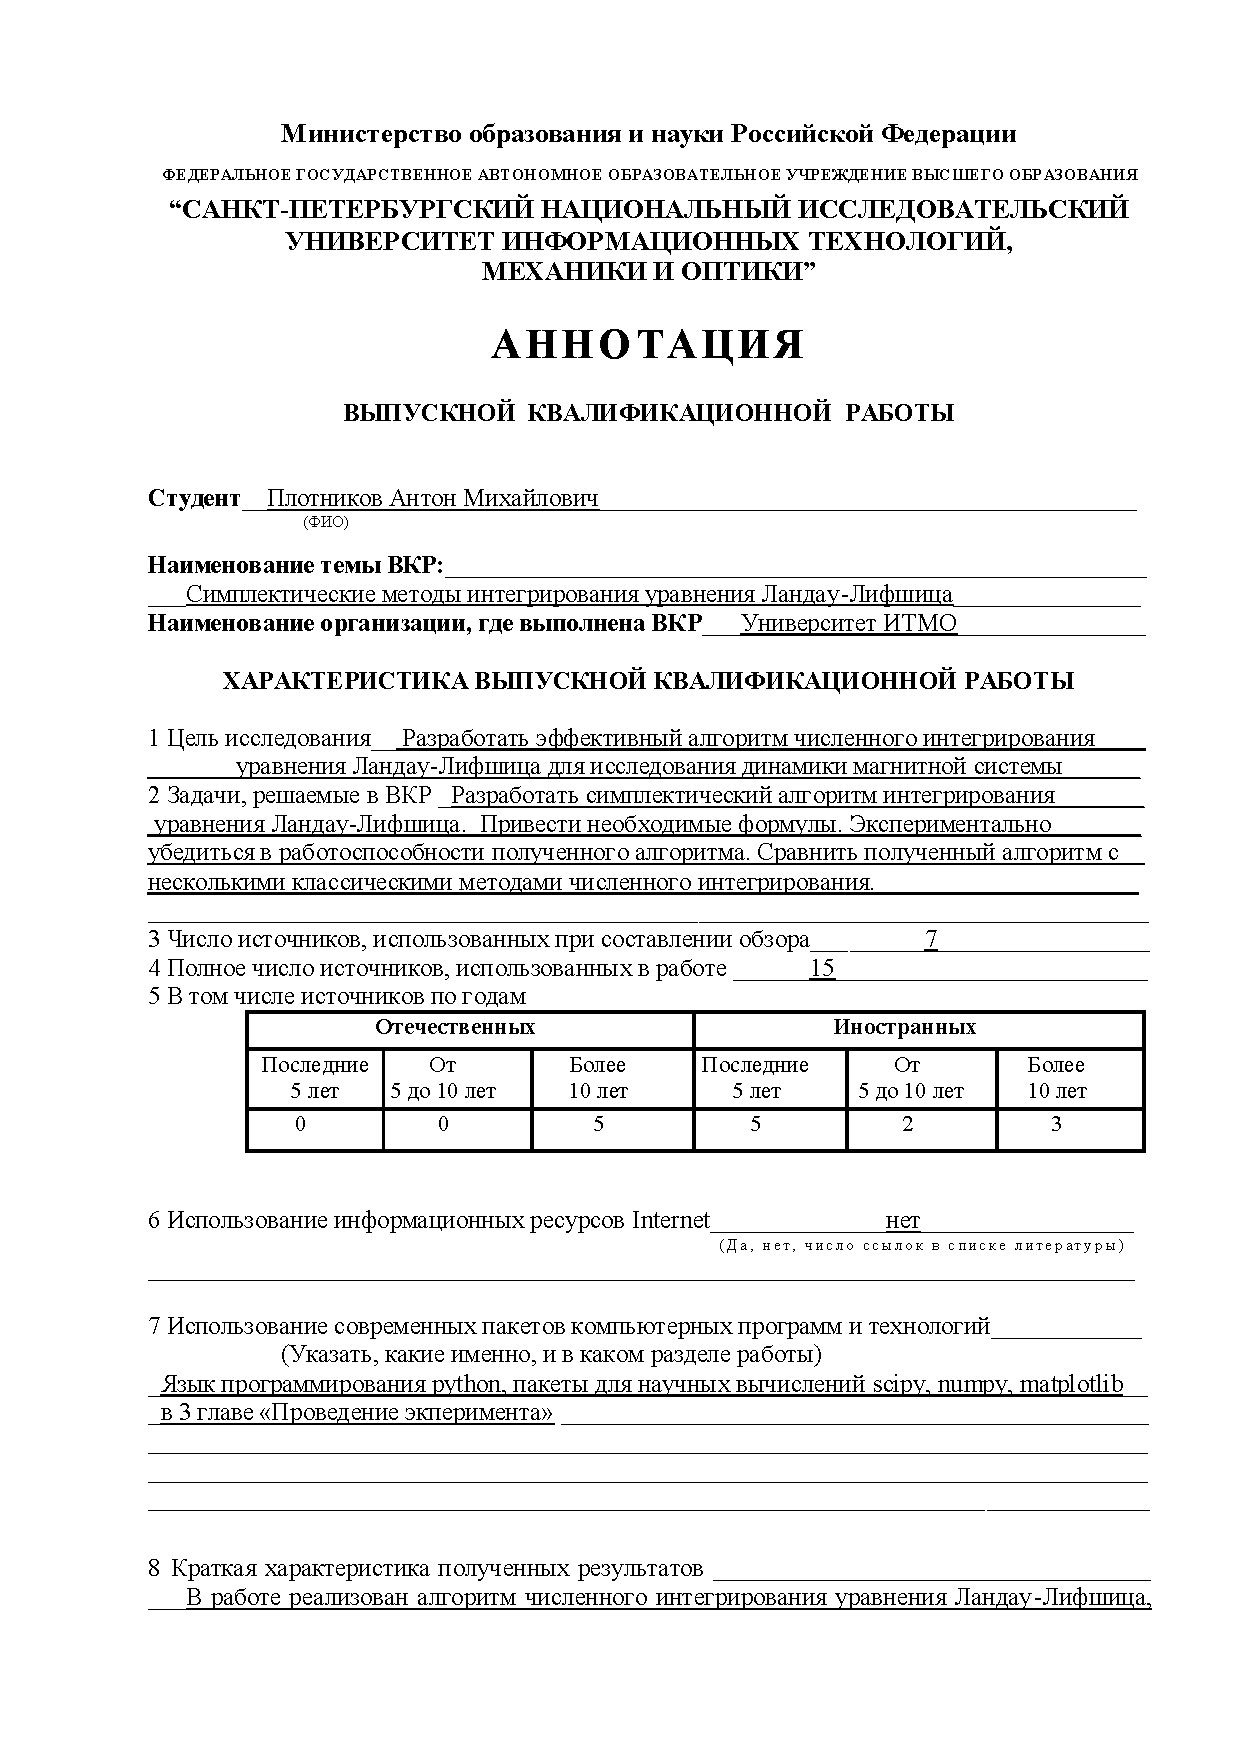
\includepdf[pages=-]{anotation.pdf}
%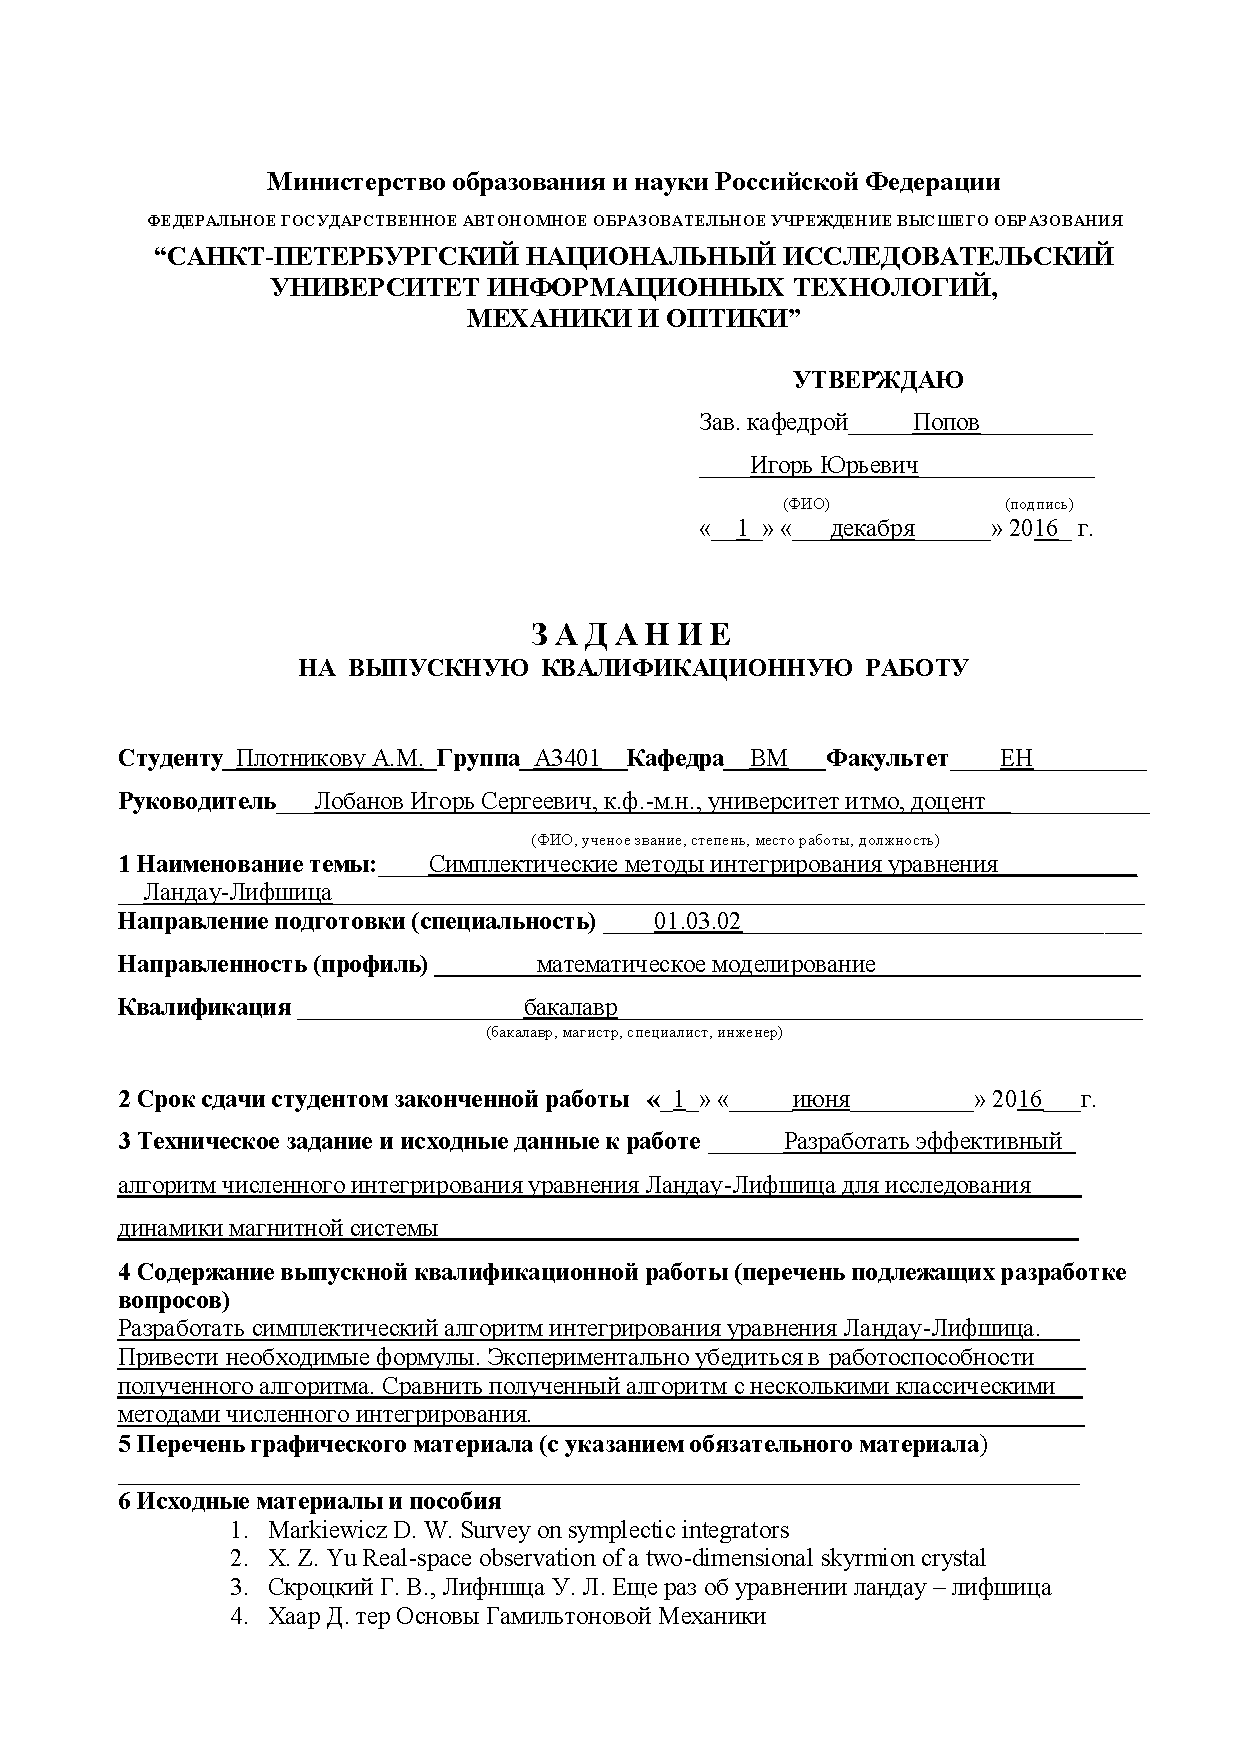
\includepdf[pages=-]{task.pdf}
\setcounter{page}{4}

\tableofcontents
\newpage

\likechapter{УСЛОВНЫЕ ОБОЗНАЧЕНИЯ}
%\newcommand*{\heff}{\ensuremath{\mathbf{H}_{eff}}}
\newcommand*{\heff}{\ensuremath{\mathcal{H}}}
\newcommand*{\Sn}{\ensuremath{\mathbf{S}^{[n]}}}

\begin{itemize}
    \item $\Sn$ --- элемент вектора (столбец матрицы) $S$
        индексом $n$,
    \item $a \thicksim b$ --- обозначение наличия связи между атомами решетки с
        индексами $a$ и $b$,
    \item $\mathbf{E} $ --- полная энергия системы,
    \item $\mathbf{B} $ --- магнитное поле,
    \item $\mathbf{D}^{[n,m]} $ --- вектор Дзялошинского-Мория для пары
        соседних атомов $n$ и $m$,
    \item $\mathbf{J}^{[n,m]} $ --- коэффициент межатомного взаимодействия
        между атомами $n$ и $m$,
    \item $\mathbf{K} $ --- единичный вектор направления анизотропии,
    \item $\mathrm{K0} $ --- коэффициент анизотропии,
    \item $\delta_{kn} $ --- символ Кронекера,
    \item $\mathrm{Id_n} $ --- единичная матрица ранга $n$,
    \item $\dot a $ --- производная $a$ по времени,
    \item $\left<a | b\right> $ --- скалярное произведение векторов $a$ и $b$.
\end{itemize}
\newpage


\likechapter{ВВЕДЕНИЕ}\label{ch:intro}

Последнее время часто поднимается тема магнитных скирмионов в научных работах и
публикациях. Скирмионы -- это квазичастица, представляющая собой структуру,
выстраивающуюся из спинов нескольких атомов, обзор скирмионной системы на
двумерной кристаллической решетке можно посмотреть, например в \cite{Yu2010}.
За счет стабильности (подробнее можно прочесть в статье \cite{nucleation},
опубликованной в журнале Science) и своих малых размеров (порядка 1-2
нанометров) они представляют интерес в использовании в качестве ячеек магнитной
памяти. В недавно-опубликованной статье \cite{stat-ant-dyn-prop-of-skyr},
ученые из университета Тохоку изучили динамику поведения скирмионов в
антиферромагнетиках и предсказали их поведение с учетом силы Магнуса, таким
образом поведение магнитных скирмионов можно считать потенциально управляемым.

Магнитная система описывается уравнением Ландау-Лифшица, которое крайне сложно
проинтегрировать символьно, поэтому для исследования динамики систем
скирмионных структур будет полезно вывести метод, с помощью которого можно
моделировать поведение скирмионов в динамически меняющихся условиях, например
воздействие на них точечного заряда или изменении магнитного поля, который при
этом будет достаточно эффективен и точен для наблюдения динамики системы в
''реальном времени``. Так же о такой системе известно что энергия (в
без диссипативной среде) должна сохранятся, поэтому нельзя пользоваться
обычными численными методами высоких порядков, таких как методы Рунге-Кутта,
поскольку они не гарантируют сохранений каких-либо инвариантов систем.

\newpage
В настоящей работе предлагается алгоритм сохраняющий симплектическую структуру
магнитной системы на основе симплектических методов Рунге-Кутта, для изучения
динамики системы, описанной уравнением Ландау-Лифщица.  В главе \ref{ch:survey}
дан обзор используемых в решении поставленной задачи численных методов,
напоминается уравнение Гамильтона и его свойства и уравнение Ландау-Лифшица.  В
главе \ref{ch:problem} описывается конкретная постановка проблемы и приведение
необходимых формул для использования их в приведенных в главе \ref{ch:survey}
методах.  Далее в \ref{ch:realisation} приведены результаты проведенных
экспериментов, представлены сравнительные графики зависимостей исследуемых
характеристик моделей и сравнение эффективности работы предлагаемого алгоритма
и классических алгоритмов Эйлера и Рунге-Кутта.


\chapter[КРАТКИЙ ОБЗОР МАТЕРИАЛОВ]%
{КРАТКИЙ ОБЗОР МАТЕРИАЛОВ ПО ИССЛЕДУЕМОЙ ТЕМЕ}\label{ch:survey}
\section{Уравнения Гамильтона в электродинамике}
Динамическую систему с $s$ степенями свободы можно описать с помощью $2s$
обыкновенных дифференциальных уравнений. Удобным способом записи является
запись с помощью уравнений Гамильтона
\begin{equation}\label{eq:ham-system}
    \begin{dcases}
        \dot q_k = \frac{\partial H(p, q)}{\partial p_k}\\
        \dot p_k = -\frac{\partial H(p, q)}{\partial q_k}
    \end{dcases}, \qquad k = 1\dots s.
\end{equation}

В простых случаях гамильтониан представляет собой энергию системы. Рассмотрим
автономную систему, т.е. систему гамильтониан не зависит явно от времени, тогда
\begin{equation}
    \frac{\partial H}{\partial t} = 0,
\end{equation}
легко показать что в такой системе функция Гамильтона, записанная в виде
\ref{eq:ham-system}, не меняется со временем
\begin{multline}
    \frac{d H}{dt} = \sum_j\left(\frac{\partial H}{\partial q_j}
    \dot q_j + \frac{\partial H}{\partial p_j}\dot p_j\right) + \frac{\partial
    H}{\partial t}
    =\\=
    \sum_j\left(\frac{\partial H}{\partial q_j} \frac{\partial H}{\partial p_i}
    - \frac{\partial H}{\partial p_j}\frac{\partial H}{\partial q_i} \right)
    + \frac{\partial H}{\partial t} = \frac{\partial H}{\partial t} = 0.
\end{multline}

Подробнее изучить материал можно, например, в работах
\cite[с.~123]{hamilton-mech} и \cite[с.~260]{classic-mech}.

Такие системы обычно невозможно решить в символьном виде, поэтому нужно
воспользоваться какими-нибудь численными методами.

\section{Метод Эйлера}\label{sec:sol-euler}
Наивное интегрирование методом Эйлера:
\begin{equation}
    \mathbf S_{n+1} = \mathbf S_{n} + h\Delta{\mathbf S_n},
\end{equation}
где $h$ -- скорость в методе Эйлера, а
\begin{equation}
    \Delta{\mathbf S_n} = -|\gamma|\left[\mathbf S_n \times 
    \mathbf H^{eff}\right].
\end{equation}

Убедимся на графиках в том что энергия при интегрировании методом Эйлера не
сохраняется и в том что ошибка накапливается линейно, поскольку используемый
численный метод, как сказано выше имеет 1 порядок, построив график зависимости
ошибки от времени при различном шаге. График зависимости ошибки энергии от
времени для метода Эйлера изображен на рис.~\ref{fig:eulerEnergy}.

О модели мы знаем не только то что она должна сохранять энергию, но и то что
вектора спинов находятся на единичной сфере, поэтому сумма длин всех векторов
должна сохраняться, для метода Эйлера график зависимости ошибки длины векторов
спинов от времени изображен на рис.~\ref{fig:eulerLength}.
\begin{figure}[H]
    \centering
    \begin{subfigure}[b]{0.49\textwidth}
        \centering
        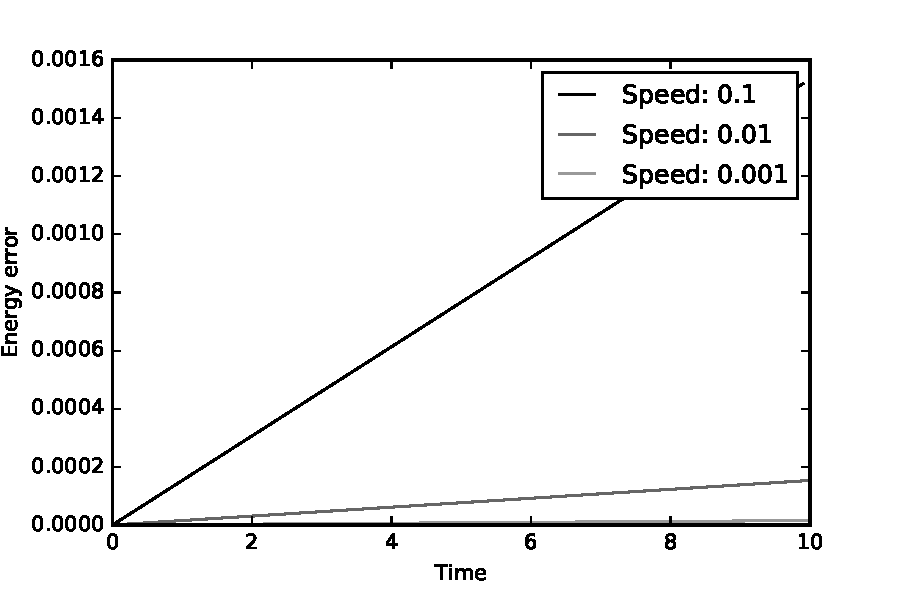
\includegraphics[width=\textwidth]{eulerEnergy.pdf}
        \caption{}
        \label{fig:eulerEnergy}
    \end{subfigure}
    \begin{subfigure}[b]{0.49\textwidth}
        \centering
        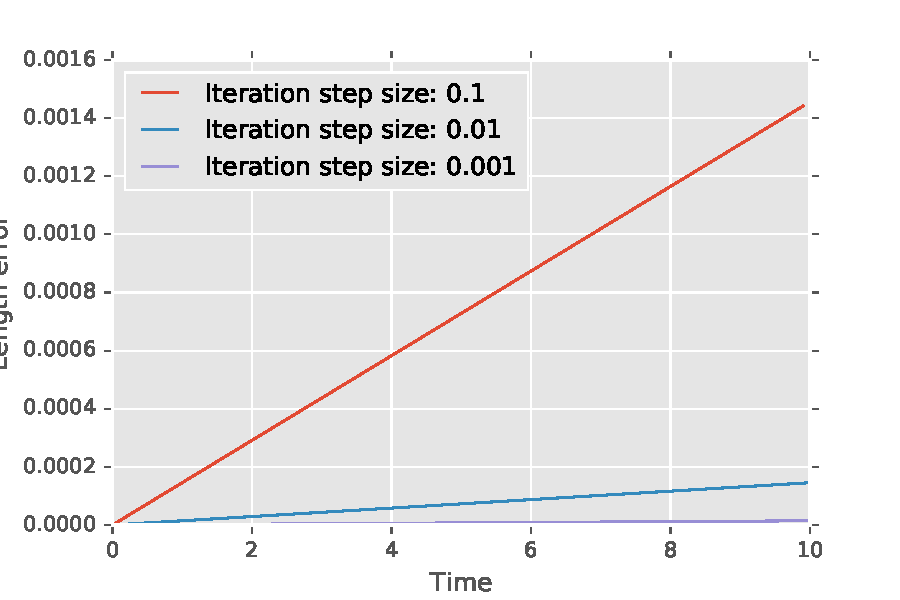
\includegraphics[width=\textwidth]{eulerLength.pdf}
        \caption{}
        \label{fig:eulerLength}
    \end{subfigure}
    \caption{(а) График зависимости ошибки энергии для метода Эйлера;
        (б) График зависимости ошибки суммы длин векторов спинов для
        метода Эйлера.}
\label{fig:euler-errors}
\end{figure}

%Для сохранения длины спинов можно на каждой итерации нормировать все вектора из
%$\mathbf S$.

%, тогда графики будут выглядеть как  и
 %для энергии системы и проекции векторов на
%направление магнитного поля соответственно.

\section{Метод Рунге-Кутта}
Также широко популярен класс численных методов решения задачи коши именуемыми
методами Рунге-Кутта.

Пусть есть задача коши \ref{eq:koshi}, тогда
в общем виде итерационная схема неявного метода Рунге-Кутта имеет вид:
\begin{figure}[h]
    \renewcommand{\arraystretch}{1.2}
    \centering
    \begin{tabular}{c|ccc}
        $c_1$    & $a_{11}$ & $\ldots$ & $a_{1s}$ \\
        $\vdots$ & $\vdots$ & $\ddots$ & $\vdots$ \\
        $c_s$    & $a_{11}$ & $\ldots$ & $a_{ss}$ \\ \hline
                 & $b_{1}$  & $\ldots$ & $b_{s}$ \\
    \end{tabular}
    \caption{Таблица для общего вида}
\label{tab:tableau_basic}
\end{figure}

\begin{equation}\label{eq:rk-schema}
    y_{n+1} = y_n + h\sum_{j=1}^s b_j f(x_n+c_jh, \xi_j)
\end{equation}
где $\xi$ вычисляется из нелинейного уравнения
\begin{equation}\label{eq:rk-not-linear}
    \xi_j = y_n + h\sum_{i=1}^{s}a_{ji} f(x_n+c_jh, \xi_i)
\end{equation}

Коэффициенты $c_i$, $a_ij$ и $b_i$ вычисляются из разложения функций $y_n,
f$ в ряд Тейлора и приравнивания коэффициентов при степенях $h^{(p-1)}$ к нулю,
где $p$ -- порядок степени аппроксимации схемы. Подробнее
см.~\cite[стр. 75]{chilsl-metodi}.

В данной работе рассматривается неявный метод Рунге-Кутта
второго порядка, имеющий второй порядок точности,
он же метод Гаусса-Лежандра-Рунге-Кутта. Для него
таблица \ref{tab:tableau_basic} выглядит как таблица \ref{tab:gauss-lagr}.

\begin{figure}[h]
    \renewcommand{\arraystretch}{1.8}
    \centering
    \begin{tabular}{c|cc}
        $\frac12 - \frac{\sqrt3}6$ & $\frac14$                  & $\frac14 - \frac{\sqrt3}6$ \\
        $\frac12 + \frac{\sqrt3}6$ & $\frac14 + \frac{\sqrt3}6$ & $\frac14$ \\ \hline
                                   & $\frac12$                  & $\frac12$
    \end{tabular}
    \caption{Таблица для метода Гаусса-Лагранжа-Рунге-Кутта}
\label{tab:gauss-lagr}
\end{figure}


\section{Метод Ньютона}

Уравнение \ref{eq:newton-needed-form}, это уравнение на нули следующей функции
\begin{equation}
    F^{[n],k}_j(\xi) = \Sn_k + h\sum_{i=1}^s a_{j,i} \left[ \xi_i^{[n],k}
    \times \nabla_{\xi^{[n],k}_i} \mathbf E(\xi) \right] -
    \xi^{[n],k}_j = 0
\end{equation}
в системе \ref{eq:newton-needed-form} $\xi$ зависит от номера шага $k$, индекс
которого можно опустить, поскольку рассматривается только один шаг.

Так же необходимо вычислить производную функции $F(x)$:
\begin{multline}
    \nabla_{\xi^{[m]}} \left[\xi^{[n]} \times \heff^{[n]}(\xi)\right]
    =\\=
    \nabla_{\xi^{[j]}} \xi^{[i]} \times \heff^{[n]}(\xi) + \xi^{[i]} \times
    \nabla_{\xi^{[j]}}\heff^{[i]}(\xi)
    =\\=
    \nabla_{\xi^{[j]}} \xi^{[i]} \times \left(A\xi^{[i]} + \mathbf B\right) +
    \xi^{[i]} \times
    \nabla_{\xi^{[j]}}\left(A\xi^{[i]} + \mathbf B\right)
    =\\=
    \delta_{i,j} \mathrm{Id}_3
    \times \left(\heff^{[i]}(\xi) \times \heff^{[i]}(\xi)\right) +
    \xi^{[i]} \times \left(
    A^{[i,j]} \right)
\end{multline}
\begin{equation}
    \nabla_{\xi_i^{[m]}}F^{[n]}_j(\xi) = ha_{j,i}\nabla_{\xi_i^{[m]}}\left(
    \xi_i^{[m]} \times \nabla_{\xi_i^{[m]}}\mathbf E [\xi_i] \right) =
    \delta_{i,j}\delta_{n,m} \mathrm{Id}_3
\end{equation}
где $\mathrm{Id}_3$ -- единичная матрица с рангом 3.

\begin{remark}
    Тут и далее под векторным произведением матрицы на вектор имеется в виду:
    \begin{equation}
        (A_1|\dots|A_n) \times B = (A_1 \times B |\dots| A_n \times B)
    \end{equation}
    где $A$ и $B$ вектора.
\end{remark}

\section{Уравнение Ландау-Лифшица}

Уравнение Ландау-Лифшица в форме Ландау-Лифшица-Гильберта описывает движение
векторов намагниченности в кристаллических решетках фери- и ферромагнетиков в
системе с диссипацией подробнее см.~\cite{lan-lif-again}.
\begin{equation}\label{eq:lan-lif-full}
    \frac{\partial \mathbf{S}}{\partial t} = - |\gamma|\left[\mathbf{S}\times
    \heff\right]-
    |\gamma|\lambda S \times \left( \mathbf S \times \heff \right),
\end{equation}
тут $\gamma$ некоторая феноменологическая постоянная,
$\heff$ -- эффективное магнитное поле, которое выражается через градиент
энергии $\mathbf E$ (вид гамильтониана см.~\cite[с. 2]{Hagemeister2015}):
\begin{equation}
    \heff = -\nabla \mathbf E \label{eq:heff-def}.
\end{equation}



\chapter{ПОСТАНОВКА ПРОБЛЕМЫ}\label{ch:problem}
\section{Уравнение Ландау-Лифшица}
Рассмотрим систему описываемую уравнением Ландау-Лифшица
(\ref{eq:lan-lif-full}).
Второе слагаемое в этом уравнении является диссипативным членом.
В данной работе исследуются симпликтические методы интегрирования уравнения
Ландау-Лифшица с целью сохранения полной энергии системы, поэтому далее
уравнение (\ref{eq:lan-lif-full}) будет рассматриваться как уравнение для
бездиссипативной среды и выглядеть следующим образом:
\begin{equation}\label{eq:lan-lif}
	\frac{d \mathbf S}{d t} = - |\gamma|[\mathbf S\times \heff].
\end{equation}

Будем рассматривать систему вклад в энергию которой вносят:
\begin{itemize}
    \item $\sum\limits_n \Braket{\mathbf B | \Sn}$ -- внешнее магнитное поле
    \item $\mathrm{K_0} \sum\limits_n \left| \Braket{\mathbf K | \Sn }
        \right|^2 $
        -- анизотропия, где $\mathrm{K_0}$ -- линейный вклад в анизотропию и
        $\mathbf K$ -- единичный вектор направления вектора анизотропии
    \item $\sum\limits_{n\thicksim m} J^{[n,m]}$ -- межатомное взаимодействие
        между атомами $n$ и $m$
    \item $\Braket{\mathbf D^{[n,m]} | \left(\Sn \times
        \mathbf S^{[m]}\right) }$ -- вектор Дзялошинского-Мория между атомами
        $n$ и $m$
\end{itemize}
\begin{multline}
    \mathbf E = -\sum_n \Braket{\mathbf B | \Sn} - \mathrm{K_0} \sum_n
    \left| \Braket{\mathbf K | \Sn } \right|^2
    -\\-
    \sum_{n\thicksim m} J^{[n,m]} \Sn - \sum_{n\thicksim m}
    \Braket{\mathbf D^{[n,m]} | \left(\Sn \times \mathbf S^{[m]}\right)}.
\end{multline}

Для удобства дальнейших расчетов перепишем в эффективное магнитное поле
(\ref{eq:heff-def}) в виде
\begin{equation}
    \heff^{[n]} = \nabla_{\mathbf S^{[n]}}\mathbf{E}
\end{equation}
где
\begin{multline}
    \nabla_{\mathbf S^{[n]}}\mathbf E
    =\\=
    \nabla_{\mathbf S^{[n]}} \left({%
    -\sum_n \Braket{\mathbf S^{[n]} | \mathbf K \mathrm{K_0}\Braket{\mathbf K |
    \mathbf S^{[n]}}} - \frac12 \Braket{\sum_n \mathbf S^{[n]} |
    \sum_{n\thicksim m} J^{[n,m]}\mathbf S^{[m]}}
    }\right.-\\-\left.{%
    \frac12\Braket{\mathbf S^{[n]} | \sum_{n\thicksim m} \mathbf S^{[n]} \times
    \mathbf D^{[n,m]}}
    -
    \sum_n \Braket{\mathbf B | \mathbf S^{[n]}}
    }\right)
    =\\=
    \underbrace{%
    -2\mathrm{K_0}\mathbf K \Braket{\mathbf K | \mathbf S^{[n]}}
    -
    \sum_{n\thicksim m}J^{[n,m]}\mathbf S^{[m]} - \sum_{n\thicksim m}
    \mathbf S^{[m]}\times \mathbf D^{[n,m]}
    }_{A\mathbf S^{[n]}}
    -
    \mathbf B.
\end{multline}
Для удобства дифференцирования далее будем рассматривать уравнение
(\ref{eq:heff-def}) в виде
\begin{equation}
    \heff^{[n]}=\nabla_{\mathbf S^{[n]}}\mathbf E = A\mathbf S^{[n]} - \mathbf B.
\end{equation}

\section{Симплeктический интегратор}\label{sec:symplectic-integrator}
Чтобы воспользоваться симплектическим методом нужно убедиться в том,
что энергия в системе, описанной уравнением Ландау-Лифшица \ref{eq:lan-lif},
действительно должна сохраняться. Для этого посмотрим на ее дифференциал и
убедимся что он равен $0$.
\begin{equation}
    \frac{d\mathbf E(S(t))}{dt} =
    \left<\nabla_S \mathbf E, \dot{\mathbf S} \right> =
    \left< \nabla_\mathbf S \mathbf E, \gamma \mathbf S \times \nabla_S \mathbf E
    \right> = 0
\end{equation}

Так же Гамильтониан должен быть представлен в симплектической форме:
\begin{equation}\label{eq:ham_sym_form}
    \begin{cases}
        \dot q^{[n]} = \dfrac{\partial \mathbf E}{\partial p^{[n]}}
        \\
        \dot p^{[n]} = - \dfrac{\partial \mathbf E}{\partial q^{[n]}}
    \end{cases}
\end{equation}

Поскольку $\mathbf S^{[n]}$ всегда единичный вектор в $\mathds R^3$
,в определенной фиксированной точке, то его состояние можно однозначно
определить парой координат в ортогональном базисе, например в сферических
координатах или с помощью длин ортогональных векторов на сфере.
Таким образом можно ввести новый базис для
каждого атома в решетке и представить $\mathbf S^{[n]}$
следующим образом:
\begin{equation}
    \mathbf S^{[n]} = \mathbf S^{[n]}(q^{[n]}, p^{[n]})
\end{equation}

Итак необходимо убедиться в эквивалентности:
\begin{equation}\label{eq:is_ham_split_eq}
    \mathbf S^{[n]} = |\gamma| \mathbf S^{[n]}\times \nabla_{\mathbf S^{[n]}}
    \mathbf E
    \overset{?}{\Leftrightarrow}
    \begin{cases}
        \dot q^{[n]} = \frac{\partial \mathbf E}{\partial p^{[n]}}
        \\
        \dot p^{[n]} = -\frac{\partial \mathbf E}{\partial p^{[n]}}
    \end{cases}
\end{equation}

Для удобства расчетов далее пологается $\gamma=1$. Если есть необходимость
задать эту консанту отличной от $1$, то можно переопределинь энергию $\mathbf
E$ так, чтобы внести в нее эту поправку, тогда будут верны все ниже указанные
расчеты.

Посчитаем производную по времени у Гамильтониана в симплектической
форме
\begin{multline}
    \dot{\mathbf S}^{[n]} = \frac{d}{dt}\mathbf S^{[n]}(q^{[n]}(t),p^{[n]}(t))=
    \frac{\partial \mathbf S^{[n]}}{\partial q^{[n]}} \cdot \dot q^{[n]} +
    \frac{\partial \mathbf S^{[n]}}{\partial q^{[n]}}
    =\\=
    \frac{\partial \mathbf S^{[n]}}{\partial q^{[n]}}
    \frac{\partial \mathbf E}{\partial p^{[n]}}
    -
    \frac{\partial \mathbf S^{[n]}}{\partial p^{[n]}}
    \frac{\partial \mathbf E}{\partial q^{[n]}}
    =
    \left|\begin{matrix}
        \Sn & \frac{\partial \Sn}{\partial q^{[n]}} &
        \frac{\partial \Sn}{\partial p^{[n]}}
        \\
        1 & 0 & 0
        \\
        \frac{\partial \mathbf E}{\partial S} &
        \frac{\partial \mathbf E}{\partial q^{[n]}} &
        \frac{\partial \mathbf E}{\partial p^{[n]}}
    \end{matrix}\right| = \Sn \times \nabla_{\Sn}\mathbf E
\end{multline}
что и требовалось доказать в \ref{eq:is_ham_split_eq}.

Таким образом можно воспользоваться симплектическим методом Рунге-Кутта,
обзор которого можно посмотреть, например, в статье \citet{Markiewicz1999},
и пользоваться приводимыми там
формулами без явной записи гамильтониана в виде \ref{eq:ham_sym_form}.


Так как исследуемая система автономна, то в уравнениях \ref{eq:rk-schema},
\ref{eq:rk-not-linear}
функция $f(t_n + c_jh, \xi_j)$ принимает вид $f(\xi_j)$

Для исследуемой модели $f(x)$ есть правая часть уравнения Ландау-Лифшица
\ref{eq:lan-lif}:
\begin{equation}
    f(\xi) = -\mathbf S \times \heff(\xi) = \mathbf S \times \nabla_{\mathbf S}
    \mathbf E
\end{equation}

Тогда итерационная схема \ref{eq:rk-schema} для исследуемой
модели будет записана в виде:
\begin{gather}
    \mathbf S^{[n]}_{k+1} = \Sn_k + h\sum_{j=1}^s b_j \left[\Sn_k \times
    \nabla_{\xi^{[n],k}_j} \mathbf E^k \right]
    \\
    \xi_j^{[n], k} = \Sn_k + h\sum_{i=1}^s a_{j,i} \left[ -\xi_i^{[n],k}
    \times \nabla_{\xi^{[n],k}_i} \mathbf E^k \right]\label{eq:rk-not-linear}
\end{gather}
где
\begin{align}
    k &\text{ -- номер шага в методе Рунге-Кутта} \\
    n &\text{ -- номер узла в решетке}
\end{align}

Для вычисления каждого следующего состояния системы необходимо решить
нелинейное уравнение \ref{eq:rk-not-linear}. Для этого можно воспользоваться,
каким-нибудь численным методом, например методом Ньютона.


\section{Метод Ньютона}

Уравнение \ref{eq:newton-needed-form}, это уравнение на нули следующей функции
\begin{equation}
    F^{[n],k}_j(\xi) = \Sn_k + h\sum_{i=1}^s a_{j,i} \left[ \xi_i^{[n],k}
    \times \nabla_{\xi^{[n],k}_i} \mathbf E(\xi) \right] -
    \xi^{[n],k}_j = 0
\end{equation}
в системе \ref{eq:newton-needed-form} $\xi$ зависит от номера шага $k$, индекс
которого можно опустить, поскольку рассматривается только один шаг.

Так же необходимо вычислить производную функции $F(x)$:
\begin{multline}
    \nabla_{\xi^{[m]}} \left[\xi^{[n]} \times \heff^{[n]}(\xi)\right]
    =\\=
    \nabla_{\xi^{[j]}} \xi^{[i]} \times \heff^{[n]}(\xi) + \xi^{[i]} \times
    \nabla_{\xi^{[j]}}\heff^{[i]}(\xi)
    =\\=
    \nabla_{\xi^{[j]}} \xi^{[i]} \times \left(A\xi^{[i]} + \mathbf B\right) +
    \xi^{[i]} \times
    \nabla_{\xi^{[j]}}\left(A\xi^{[i]} + \mathbf B\right)
    =\\=
    \delta_{i,j} \mathrm{Id}_3
    \times \left(\heff^{[i]}(\xi) \times \heff^{[i]}(\xi)\right) +
    \xi^{[i]} \times \left(
    A^{[i,j]} \right)
\end{multline}
\begin{equation}
    \nabla_{\xi_i^{[m]}}F^{[n]}_j(\xi) = ha_{j,i}\nabla_{\xi_i^{[m]}}\left(
    \xi_i^{[m]} \times \nabla_{\xi_i^{[m]}}\mathbf E [\xi_i] \right) =
    \delta_{i,j}\delta_{n,m} \mathrm{Id}_3
\end{equation}
где $\mathrm{Id}_3$ -- единичная матрица с рангом 3.

\begin{remark}
    Тут и далее под векторным произведением матрицы на вектор имеется в виду:
    \begin{equation}
        (A_1|\dots|A_n) \times B = (A_1 \times B |\dots| A_n \times B)
    \end{equation}
    где $A$ и $B$ вектора.
\end{remark}


\chapter{ПРОВЕДЕНИЕ ЭКСПЕРИМЕНТА}\label{ch:realisation}
\section{Используемые технологии}

Для реализации модели~\ref{sec:model} был выбран язык программирования
\emph{python}, в связи с простотой синтаксиса и большим выбором
высокопроизводительных библиотек для математического моделирования, и модуль
для научных вычислений \emph{scipy}~\cite{scipy}, являющийся одним из самых
эффективных и популярных на момент написания работы.  Приемуществом
предлагаемого алгоритма является отсутствие в вычислениях сложных операций (с
точки зрения производительности выполнения операций на ЭВМ), в программе
использованы только матричные функции сложения, умножения модуля научных
вычислений \emph{numpy}~\cite{numpy}.  Графики и рисунки приведенные в работе
построены с использованием модуля \emph{matplotlib}~\cite{matplotlib}.

Вычисления производились на тестовом стенде с характеристиками:
\begin{itemize}
    \item ЦПУ: AMD A8-7100 Radeon R5, 4 ядра, 1800\,МГц
    \item ОС: Arch Linux, x86\_64 Linux 4.5.4-1-ARCH
    \item ЗУПВ:
        \begin{itemize}
            \item SODIMM DDR3 1600\,МГц, 4\,Гб, RMT3170ME68F9F1600
            \item SODIMM DDR3 1600\,МГц, 8\,Гб, CT102464BF160B.M16
        \end{itemize}
    \item \emph{python} 2.7.11
    \item \emph{scipy} 0.17.1
    \item \emph{numpy} 1.11.0
    \item \emph{matplotlib} 1.5.1
\end{itemize}


\section{Модель}\label{sec:model}

Модель представляет из себя двумерную кристаллическую решетку на плоском
торе. Каждый элемент решетки имеет свой спин (трехмерный единичный вектор).

Атомы на решетке имеют связь только с 4 своими ближайшими соседями,
то есть $i$ атом имеет связь с $i-1$, $i+1$, $i-x$, $i+x$ элементами,
если $x$ и $y$ задают размеры решетки, а узлы индексируются как
$index = p_x + x*p_y$, где $p_x$ и $p_y$ это положение
узла в решетке.

Между соседними атомами с индексами $i$ и $j$ установлена связь взаимодействия
Дзялошинского-Мория $\mathbf D_{i,j}$, в направлении от одного узла к другому.
Стоит отметить, что $\mathbf D_{i,j} = -\mathbf D_{j,i}$.

Основные характеристики модели:
\begin{itemize}
\item $b$ -- вектор характеризующий магнитное поле, далее для
    усовершенствования можно заменить на векторное поле, чтобы смоделировать
    поведение в неоднородной среде
\item $i$ -- сила межатомного взаимодействия
\item $\mathrm{K_0}$ -- абсолютное значение анизотропии
\item $\mathbf K$ -- направление вектора анизотропии, единичный трехмерный вектор
\item $\lambda$ -- параметр диссипации (для среды без диссипации $\lambda=0$)
\item $\gamma$ -- феноменологическая постоянная из уравнения Ландау-Лифшица
\item $x$ и $y$ -- размер решетки
\end{itemize}

Для сравнения эффективности метода, помимо самого симплектического метода
Рунге-Кутта \ref{sec:symplectic-integrator}, был реализован метод Эйлера
\ref{sec:sol-euler} и не симплектические методы Рунге-Кутта 2го и 4го порядка.


\section{Метод Эйлера}\label{sec:sol-euler}
Наивное интегрирование методом Эйлера:
\begin{equation}
    \mathbf S_{n+1} = \mathbf S_{n} + h\Delta{\mathbf S_n},
\end{equation}
где $h$ -- скорость в методе Эйлера, а
\begin{equation}
    \Delta{\mathbf S_n} = -|\gamma|\left[\mathbf S_n \times 
    \mathbf H^{eff}\right].
\end{equation}

Убедимся на графиках в том что энергия при интегрировании методом Эйлера не
сохраняется и в том что ошибка накапливается линейно, поскольку используемый
численный метод, как сказано выше имеет 1 порядок, построив график зависимости
ошибки от времени при различном шаге. График зависимости ошибки энергии от
времени для метода Эйлера изображен на рис.~\ref{fig:eulerEnergy}.

О модели мы знаем не только то что она должна сохранять энергию, но и то что
вектора спинов находятся на единичной сфере, поэтому сумма длин всех векторов
должна сохраняться, для метода Эйлера график зависимости ошибки длины векторов
спинов от времени изображен на рис.~\ref{fig:eulerLength}.
\begin{figure}[H]
    \centering
    \begin{subfigure}[b]{0.49\textwidth}
        \centering
        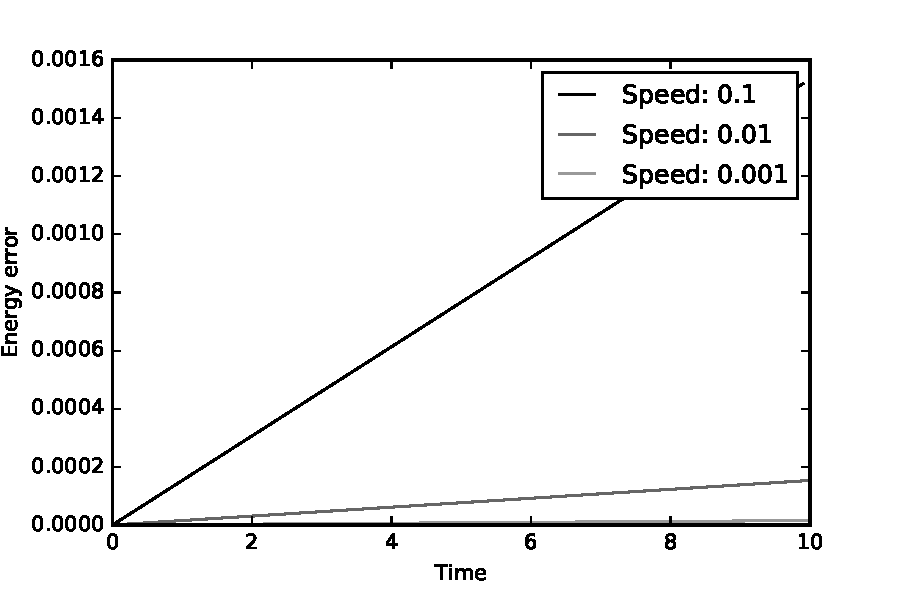
\includegraphics[width=\textwidth]{eulerEnergy.pdf}
        \caption{}
        \label{fig:eulerEnergy}
    \end{subfigure}
    \begin{subfigure}[b]{0.49\textwidth}
        \centering
        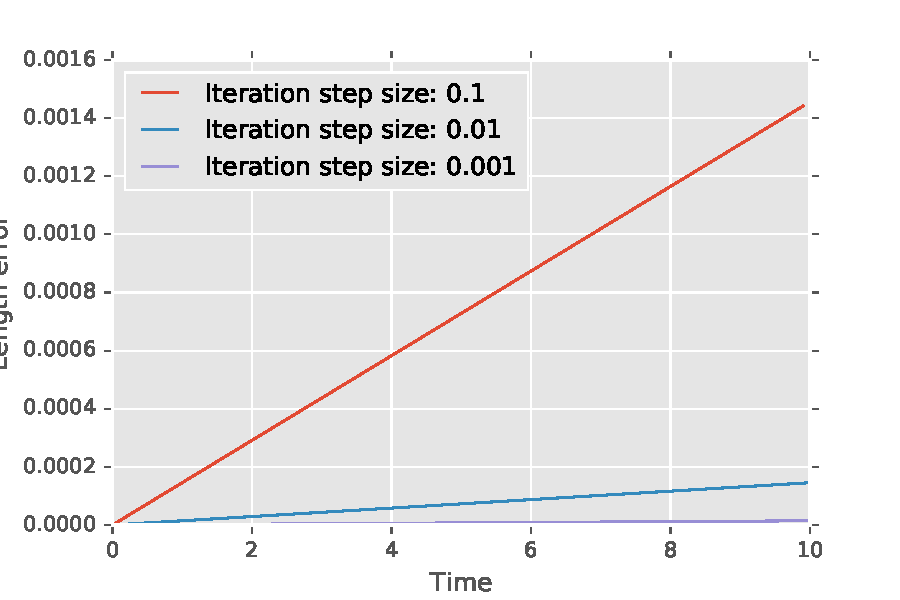
\includegraphics[width=\textwidth]{eulerLength.pdf}
        \caption{}
        \label{fig:eulerLength}
    \end{subfigure}
    \caption{(а) График зависимости ошибки энергии для метода Эйлера;
        (б) График зависимости ошибки суммы длин векторов спинов для
        метода Эйлера.}
\label{fig:euler-errors}
\end{figure}

%Для сохранения длины спинов можно на каждой итерации нормировать все вектора из
%$\mathbf S$.

%, тогда графики будут выглядеть как  и
 %для энергии системы и проекции векторов на
%направление магнитного поля соответственно.

\section{Методы Рунге-Кутта}
Построим графики тех же зависимостей для метода Рунге-Кутта второго
(рис.~\ref{fig:rk2-errors}) и четвертого (рис.~\ref{fig:rk4-errors}) порядков,
и симплектического метода Рунге-Кутта (рис.~\ref{fig:simp-rk-errors}) что и для
метода Эйлера.
\begin{figure}[H]
    \centering
    \begin{subfigure}[b]{0.49\textwidth}
        \centering
        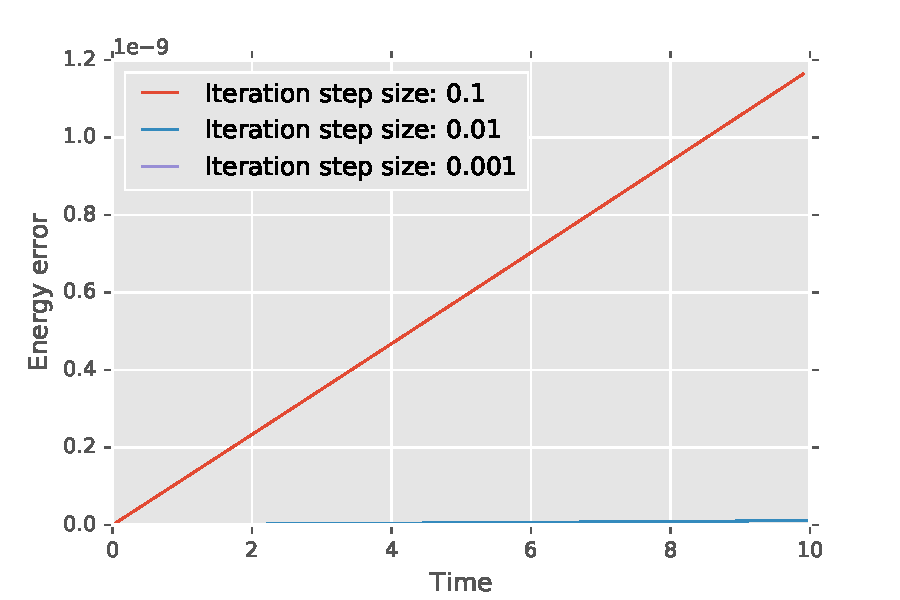
\includegraphics[width=\textwidth]{ralstonEnergy.pdf}
        \caption{}
    \end{subfigure}
    \begin{subfigure}[b]{0.49\textwidth}
        \centering
        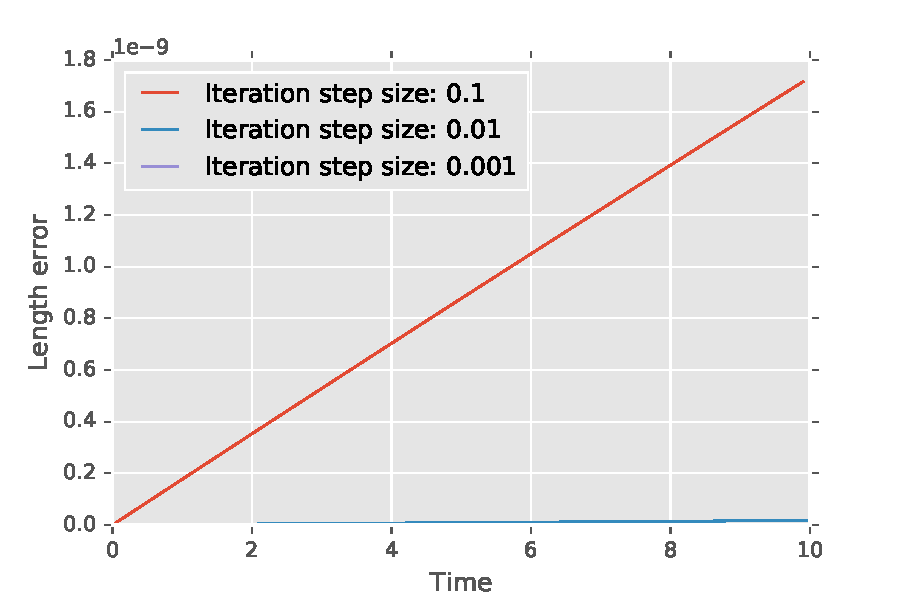
\includegraphics[width=\textwidth]{ralstonLength.pdf}
        \caption{}
    \end{subfigure}
    \caption{(а) График зависимости ошибки энергии для метода Рунге-Кутта 2го
        порядка;
        (б) График зависимости ошибки суммы длин векторов спинов для
        метода Рунге-Кутта 2го порядка.}
\label{fig:rk2-errors}
\end{figure}
\begin{figure}[H]
    \centering
    \begin{subfigure}[b]{0.49\textwidth}
        \centering
        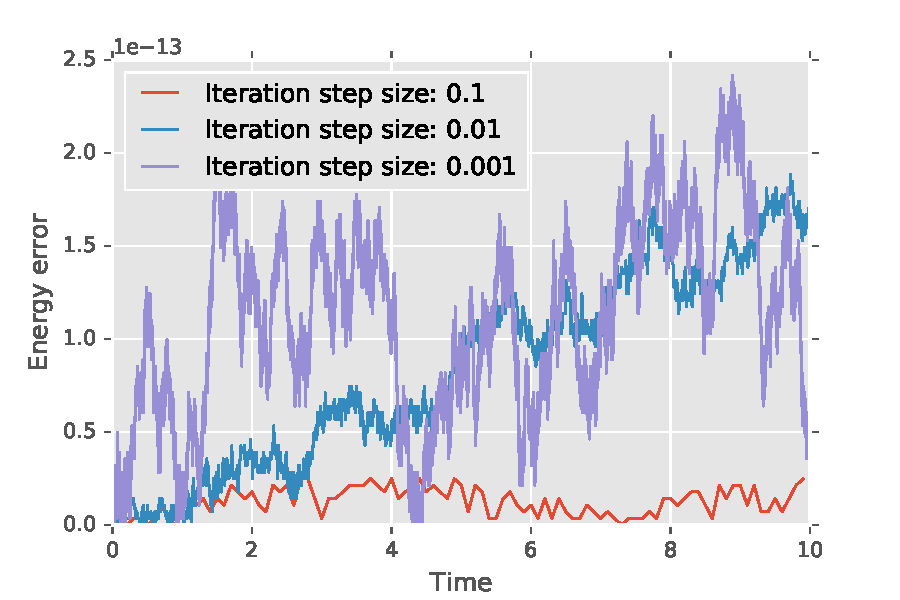
\includegraphics[width=\textwidth]{fourthEnergy.pdf}
        \caption{}
    \end{subfigure}
    \begin{subfigure}[b]{0.49\textwidth}
        \centering
        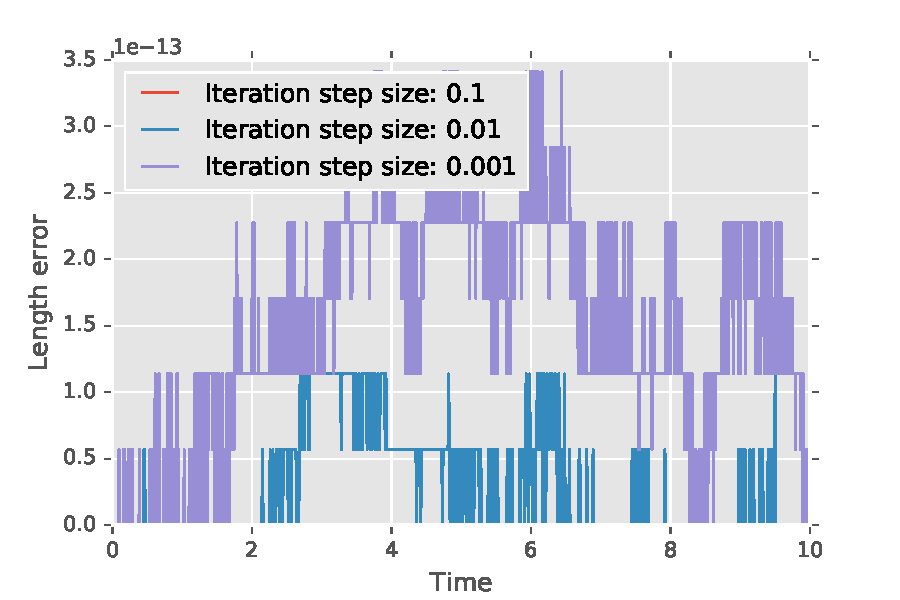
\includegraphics[width=\textwidth]{fourthLength.pdf}
        \caption{}
    \end{subfigure}
    \caption{(а) График зависимости ошибки энергии для метода Рунге-Кутта 4го
        порядка;
        (б) График зависимости ошибки суммы длин векторов спинов для
        метода Рунге-Кутта 4го порядка.}
\label{fig:rk4-errors}
\end{figure}
\begin{figure}[H]
    \centering
    \begin{subfigure}[b]{0.49\textwidth}
        \centering
        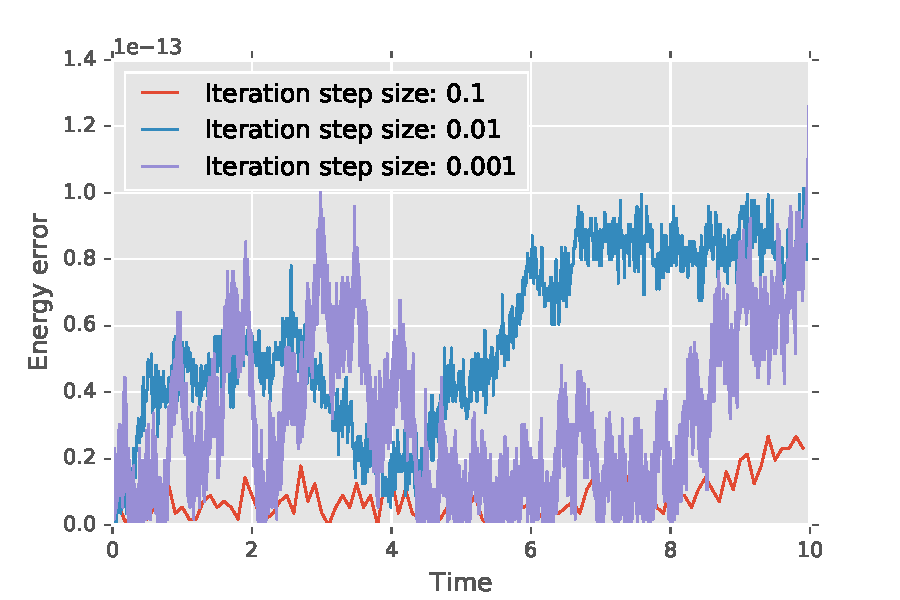
\includegraphics[width=\textwidth]{gauss2Energy.pdf}
        \caption{}
    \end{subfigure}
    \begin{subfigure}[b]{0.49\textwidth}
        \centering
        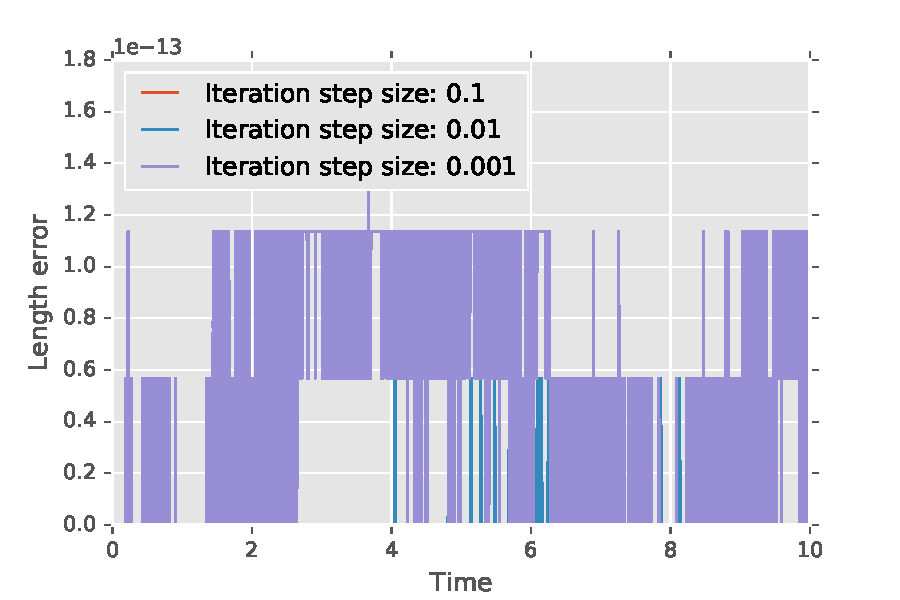
\includegraphics[width=\textwidth]{gauss2Length.pdf}
        \caption{}
    \end{subfigure}
    \caption{(а) График зависимости ошибки энергии для симплектического
        метода Рунге-Кутта;
        (б) График зависимости ошибки суммы длин векторов спинов для
        симплектического метода Рунге-Кутта.}
\label{fig:simp-rk-errors}
\end{figure}

Сравнительный график зависимости ошибки энергии, от шага интегрирования на
логарифмической шкале представленных алгоритмов, можно посмотреть на
рис.~\ref{fig:error-comparsion-energy} и ошибки суммы длин векторов на
рис.~\ref{fig:error-comparsion-length}.
\begin{figure}[H]
    \centering
    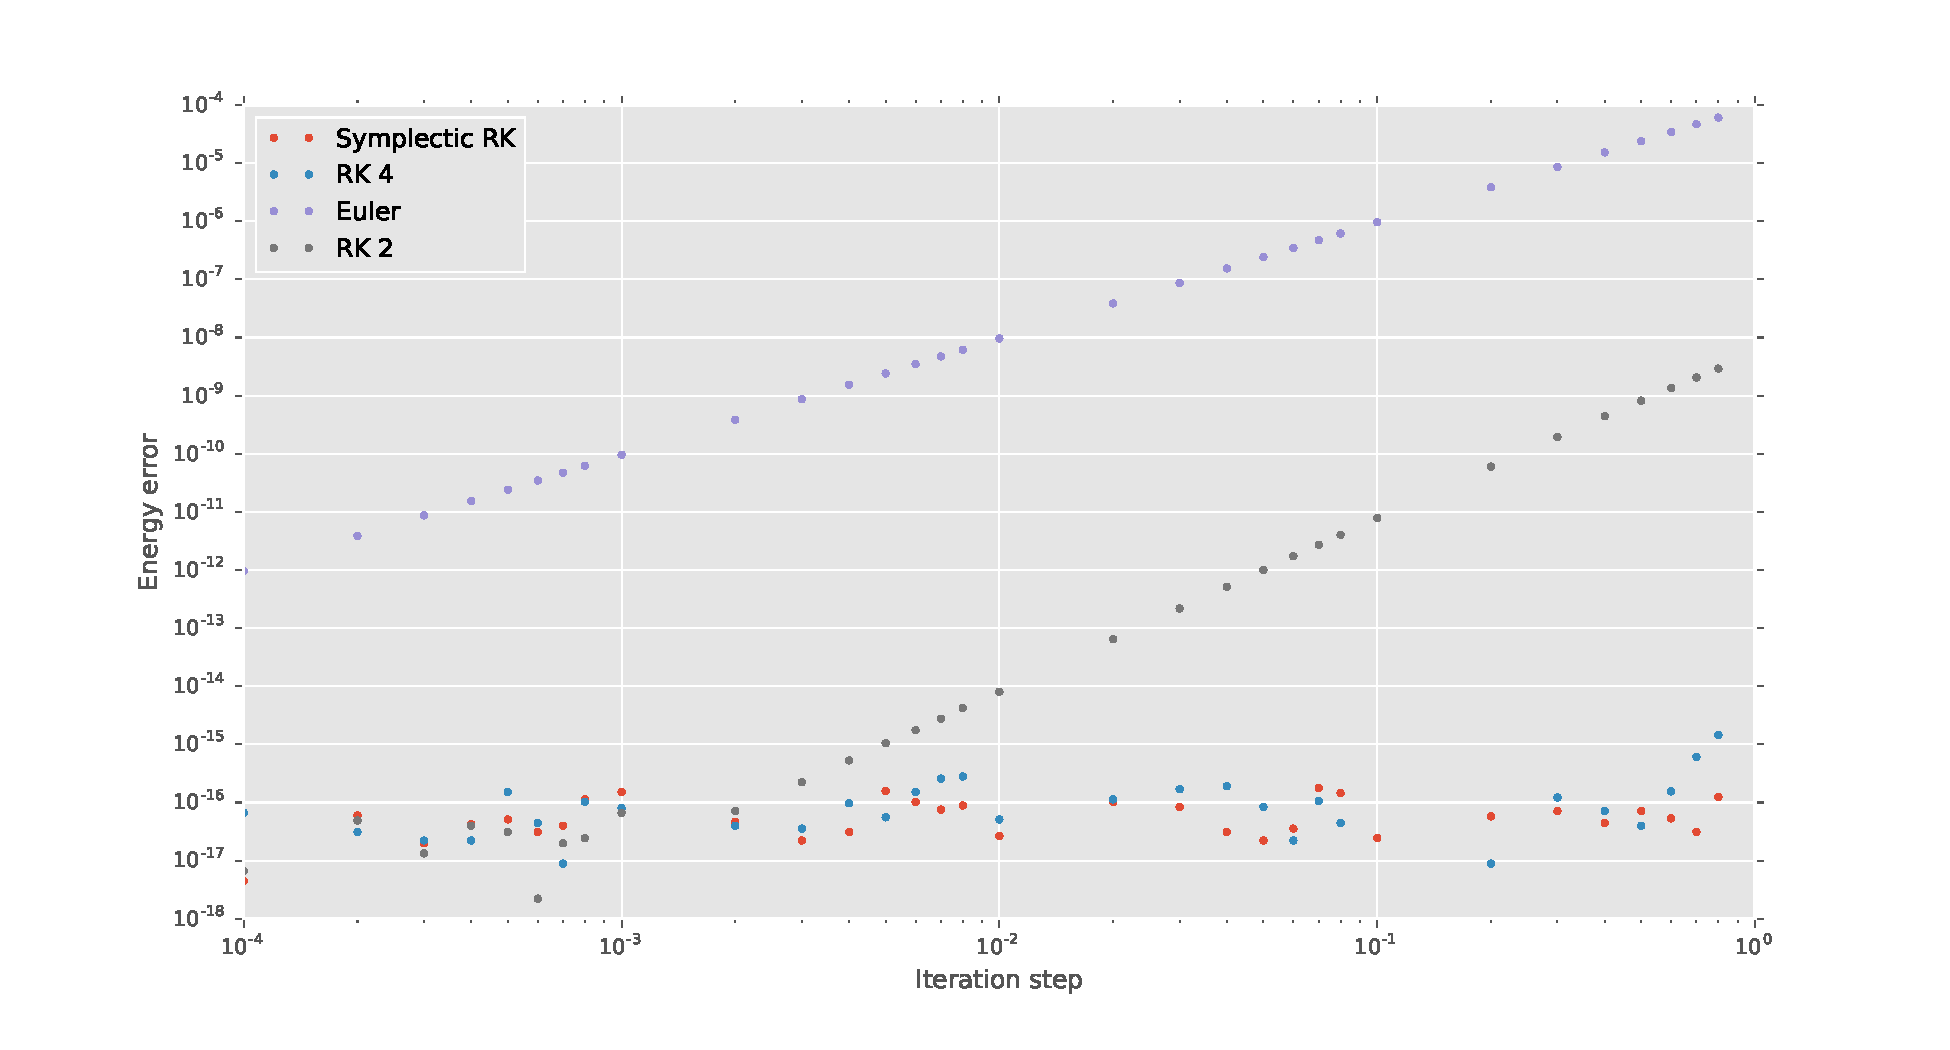
\includegraphics[width=\textwidth]{errorComparsionEnergy.pdf}
    \caption{Графики зависимости ошибки энергии от шага интегрирования на
    логарифмической шкале.}
\label{fig:error-comparsion-energy}
\end{figure}
\begin{figure}[H]
    \centering
    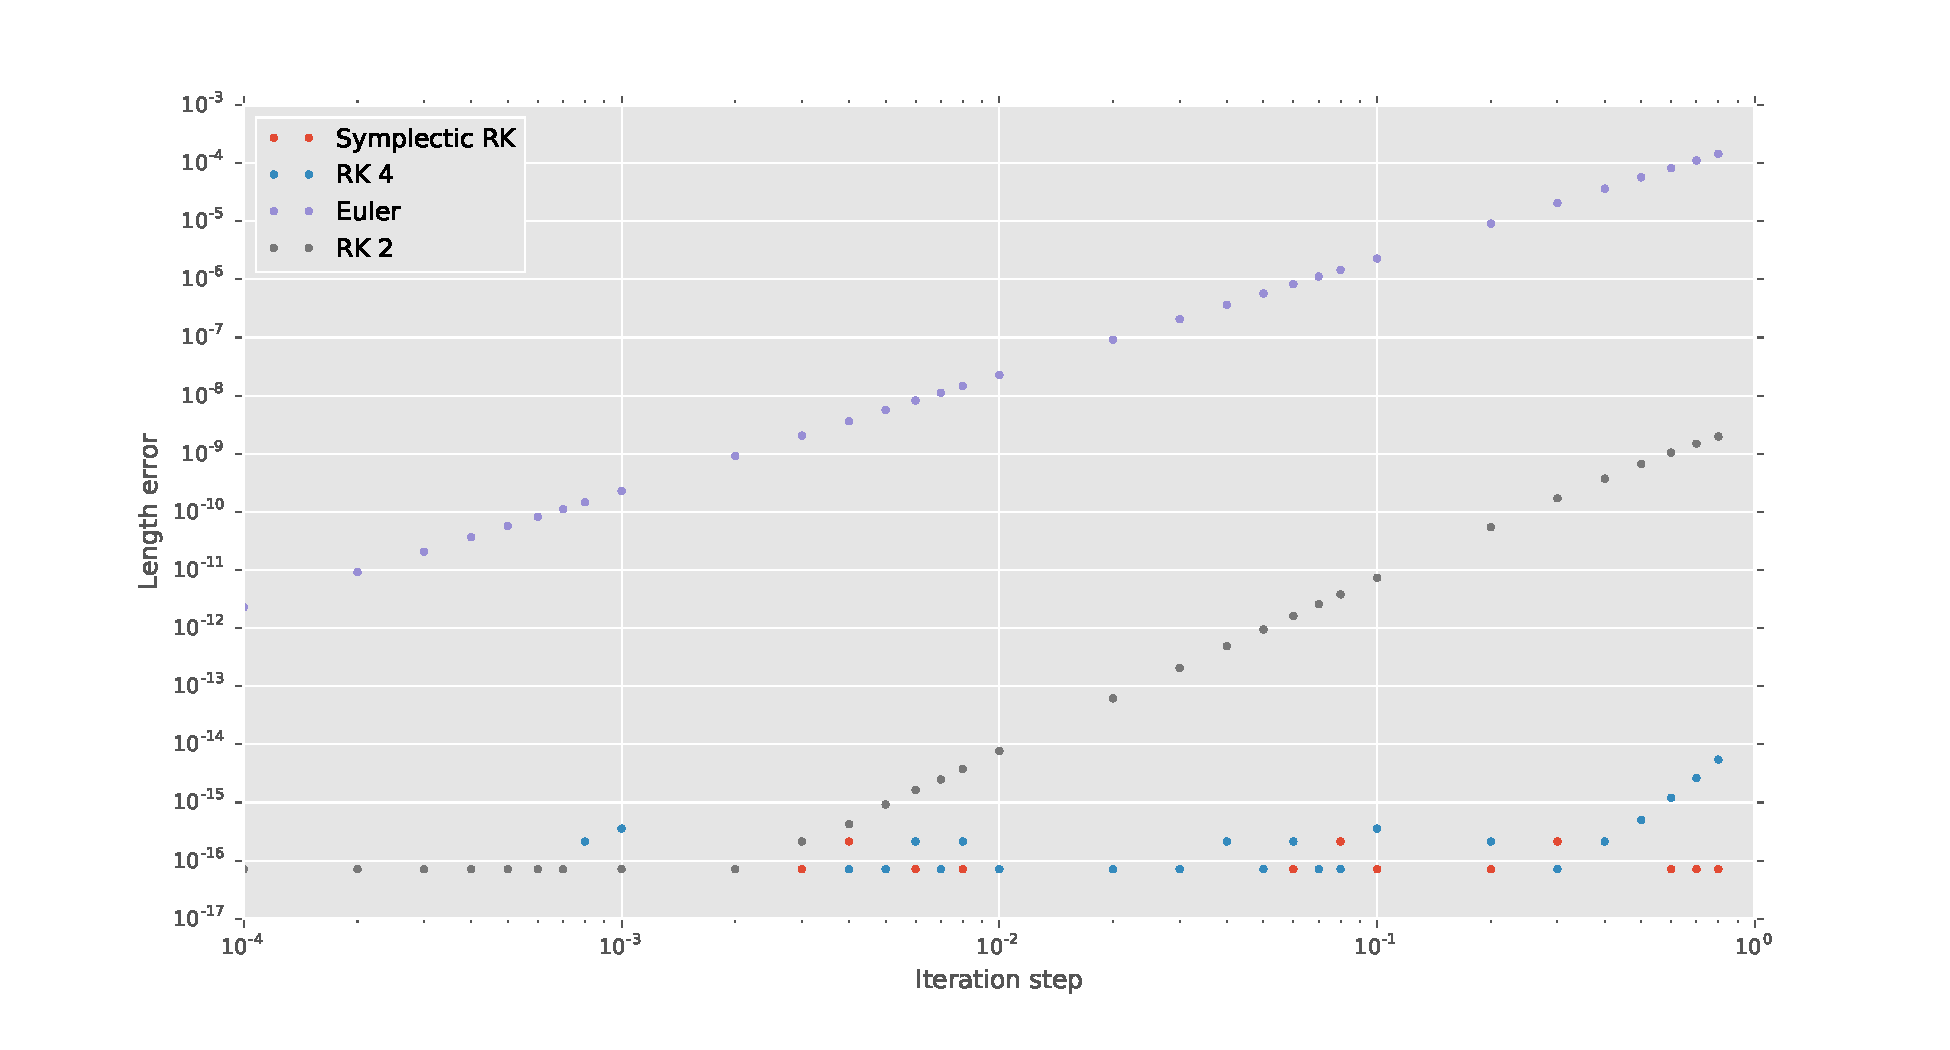
\includegraphics[width=\textwidth]{errorComparsionLength.pdf}
    \caption{Графики зависимости ошибки энергии от шага интегрирования на
    логарифмической шкале.}
\label{fig:error-comparsion-length}
\end{figure}

Сравним скорость работы алгоритмов на графиках зависимости скорости вычисления
одной итерации от размера решетки системы. Для получения следующих результатов,
алгоритмы были запущены по 1000 раз на 100 итераций с усреднением времени
выполнения одной итерации. Полученные результаты см.
рис.~\ref{fig:benchmark-speed}.
\begin{figure}[H]
    \centering
    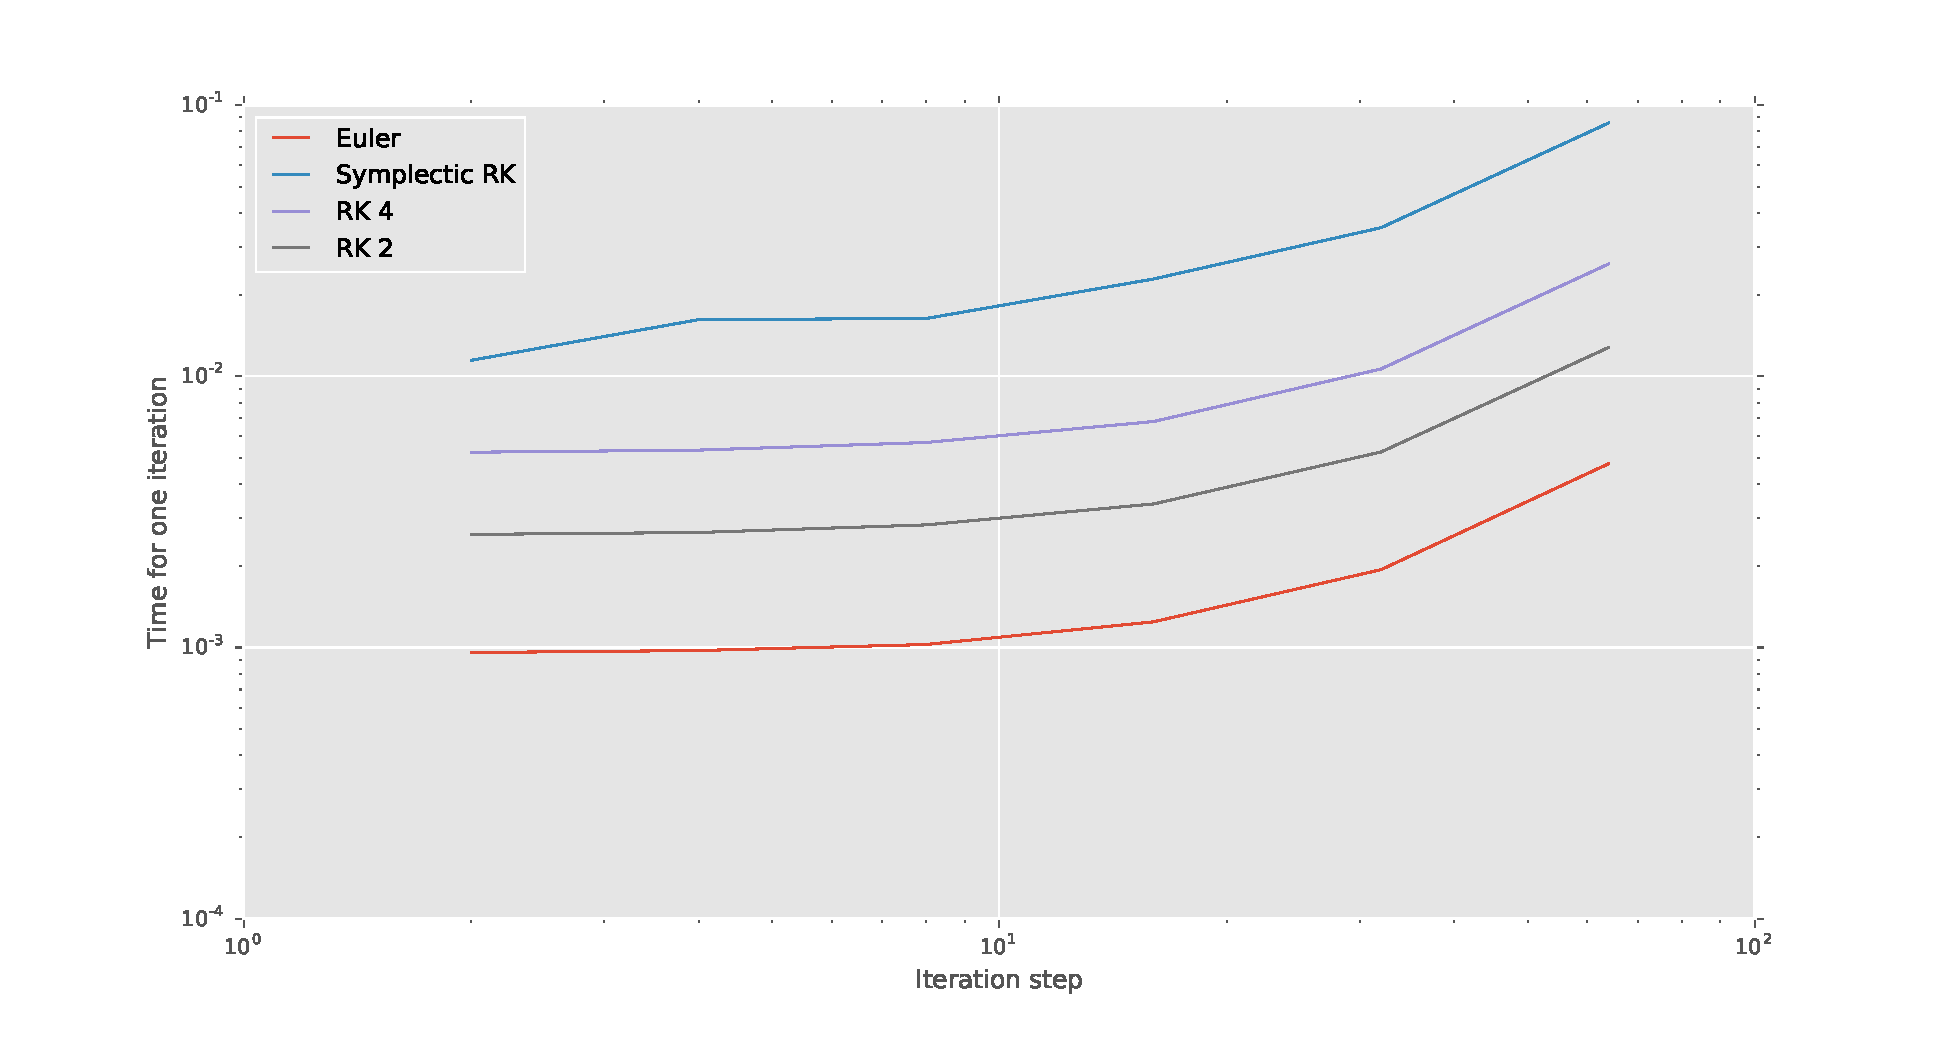
\includegraphics[width=\textwidth]{speedComparsion.pdf}
    \caption{Графики зависимости скорости вычисления одной итерации от размера
    решетки.}
\label{fig:benchmark-speed}
\end{figure}
Видно, что зависимость не линейна, на больших размерах решеток разность
скорости на одну итерацию будет не значительна, при этом предлагаемый метод
гарантирует сохранение квадратичных инвариантов на каждой итерации.


\section{Скирмион}
Для получения визуального представления скирмиона положим коэффициент
диссипации $\gamma=0$. Спины в изначальной конфигурации поля направим по
направлению магнитного поля кроме одного, направленного в противоположную
сторону, получается рисунки следующего вида~\ref{fig:skyrmion}.

\begin{figure}[H]
    \centering
    \begin{subfigure}[b]{0.49\textwidth}
        
\includegraphics[width=\textwidth]{skyrmion1.pdf}
    \end{subfigure}
    \begin{subfigure}[b]{0.49\textwidth}
        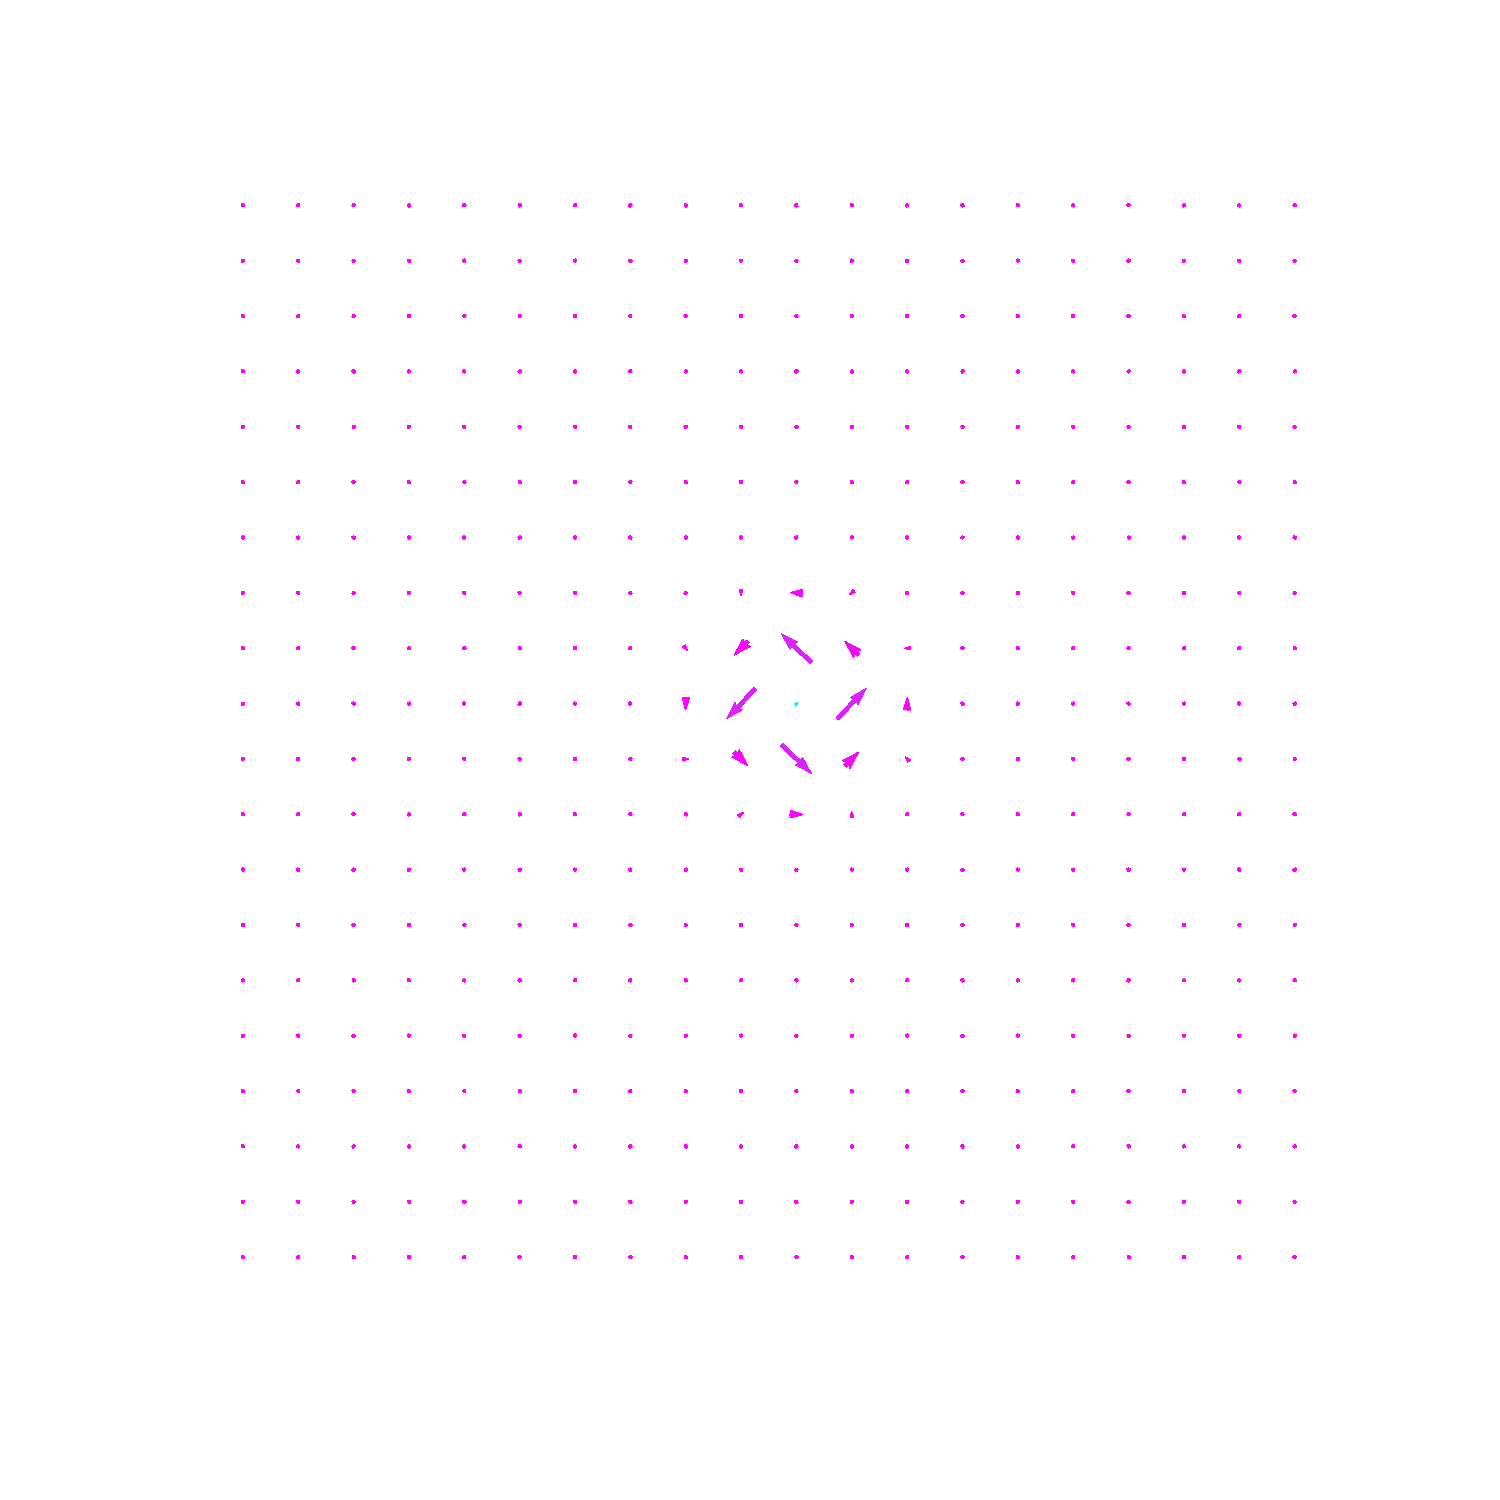
\includegraphics[width=\textwidth]{skyrmion2.pdf}
    \end{subfigure}
    \begin{subfigure}[b]{0.49\textwidth}
        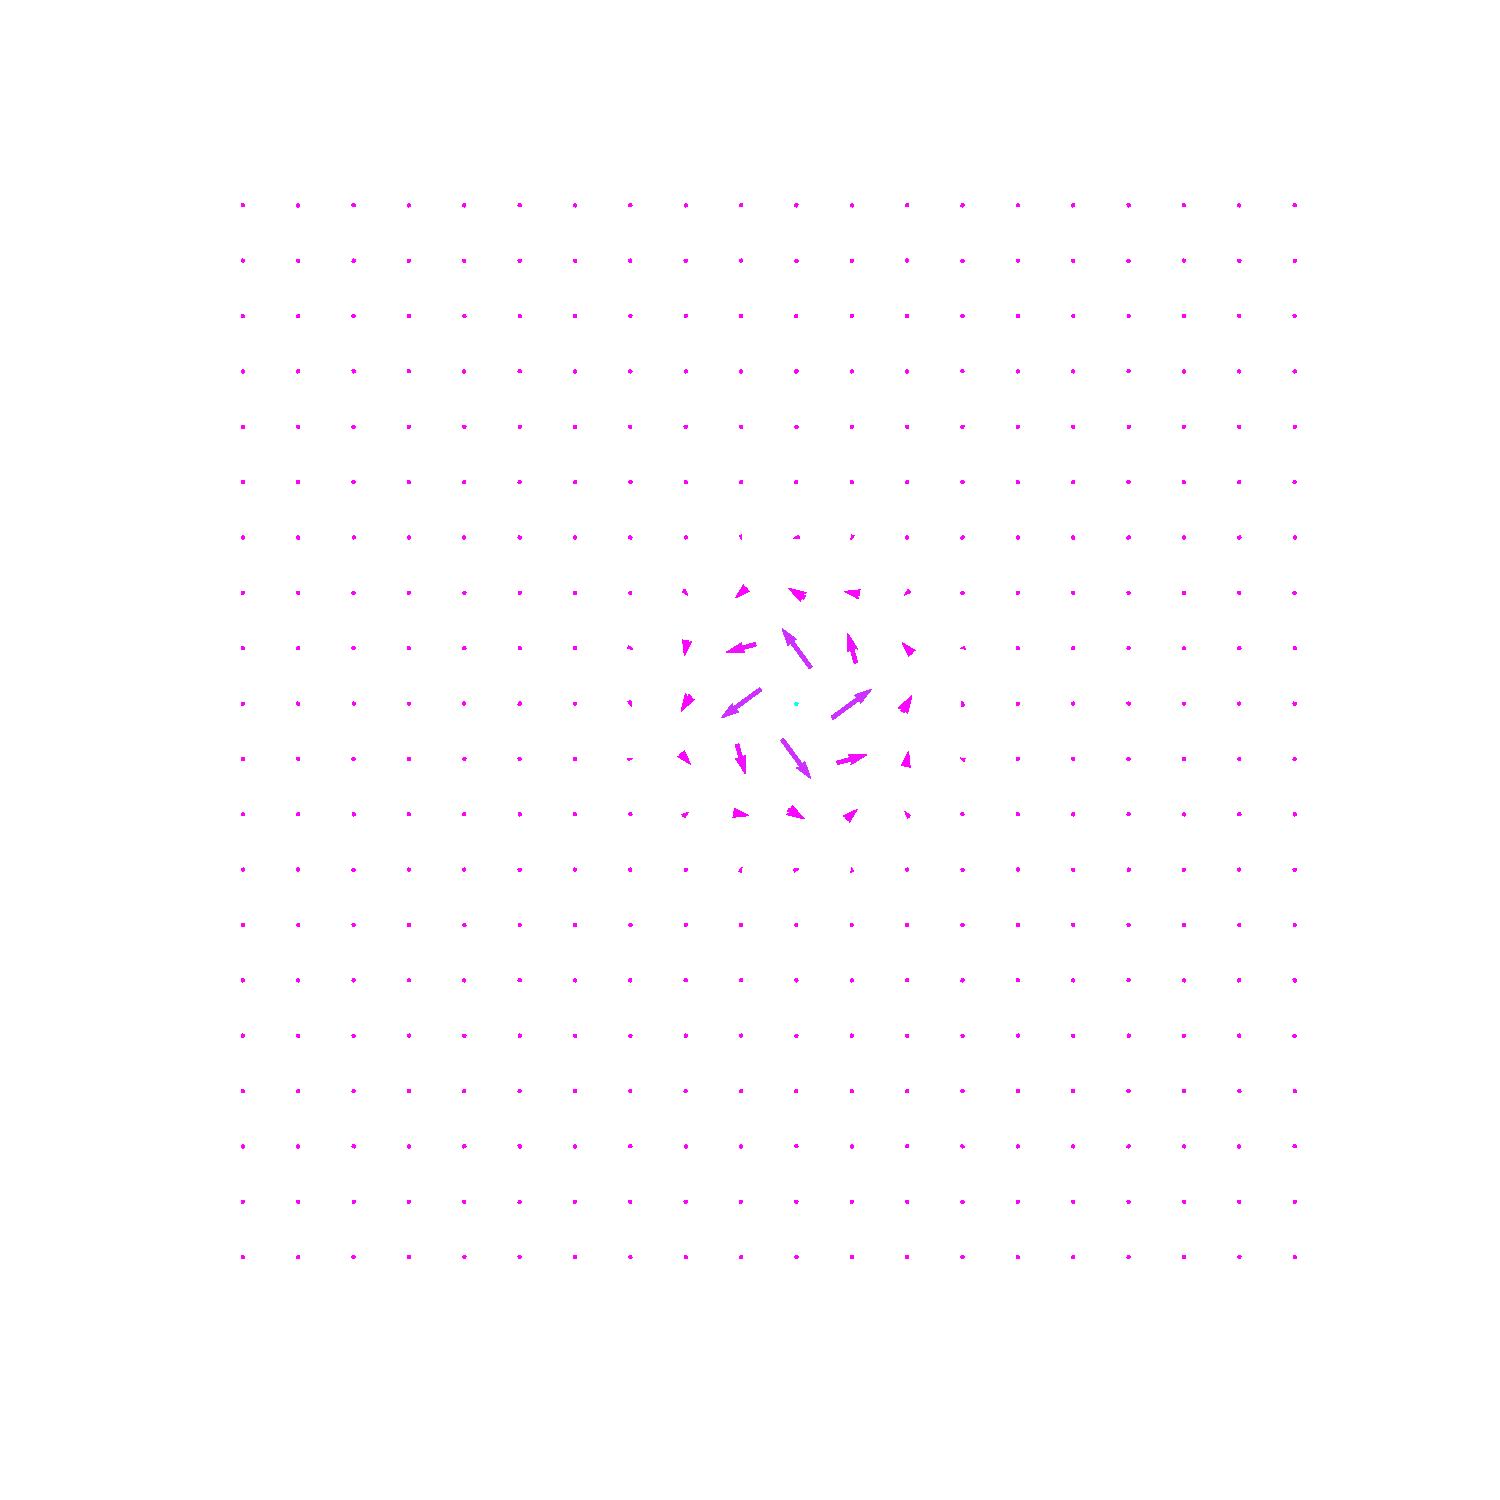
\includegraphics[width=\textwidth]{skyrmion3.pdf}
    \end{subfigure}
    \begin{subfigure}[b]{0.49\textwidth}
        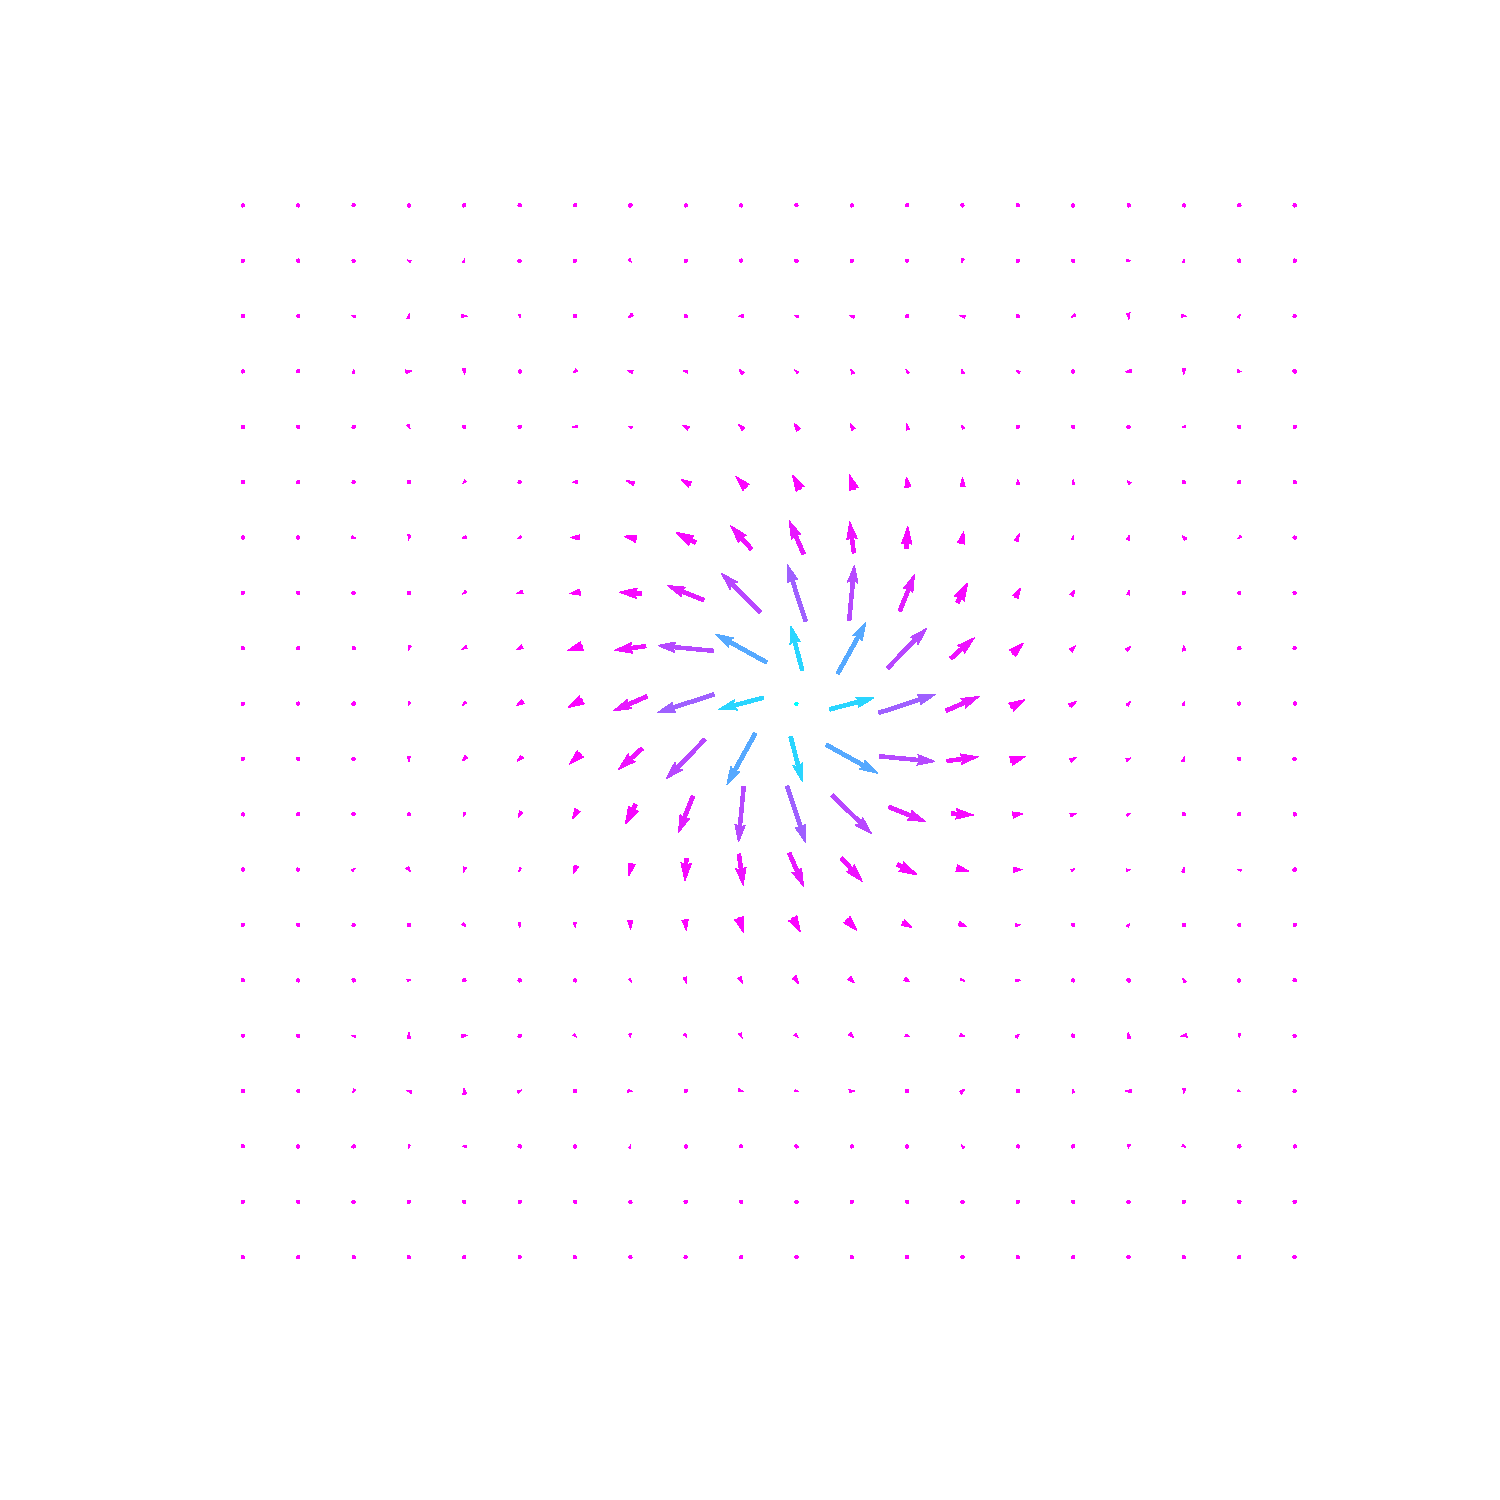
\includegraphics[width=\textwidth]{skyrmion4.pdf}
    \end{subfigure}
    \caption{Различные стадии скирмиона.}
\label{fig:skyrmion}
\end{figure}


\newpage
\likechapter{ЗАКЛЮЧЕНИЕ}

В результате работы представлен симплектический метод численного интегрирования
уравнения Ландау-Лифшица с помощью симплектического метода Рунге-Кутта и
продемонстрирована его эффективность.

Особенностью метода является, отсутствие перехода из внешней трехмерной системы
координат к локальному двумерному базису, как часто делается в подобных
задачах. Такое решение требует дополнительных ресурсов для хранения данных о
третьей координате, но при этом операции над числами производятся более
простые, в реализованной программе присутствуют только операции сложения и
умножения матриц, что происходит значительно быстрее, чем операции, например,
$\sin$ или $\cos$, которые неизбежны при переходе к сферическим координатам.


\newpage
\likechapter{СПИСОК ЛИТЕРАТУРЫ}
\printbibliography[heading=none]

\end{document}

